\documentclass{article} % Tạo một bản báo cáo
\usepackage{makecell}
\usepackage{multirow}
\usepackage{xurl} % Gói này giúp ngắt dòng URL ở bất cứ đâu, rất mạnh mẽ
\usepackage{url}
\usepackage{hyperref}
\hypersetup{
    colorlinks=true,
    linkcolor=black,
    filecolor=magenta,      
    urlcolor=blue, % Đổi màu link thành xanh dương thay vì khung
}
\renewcommand\theadfont{\bfseries}
\usepackage[utf8]{inputenc}
\usepackage[T5]{fontenc} % Để sử dụng Tiếng Việt
\usepackage[fontsize=13pt]{scrextend} % Set fontsize=13pt
\usepackage[paperheight=29.7cm,paperwidth=21cm,right=2cm,left=3cm,top=2cm,bottom=2.5cm]{geometry}% Chuẩn A4, căn lề phải, trái, trên, dưới.
\usepackage{graphicx} % Thư viện chèn ảnh
\usepackage{float} % Set vị trí chèn ảnh
\usepackage{tikz} % Thư viện tạo khung bìa
\usetikzlibrary{calc} % Thư viện tikz
\usepackage{indentfirst} % Thư viện thụt đầu dòng
\renewcommand{\baselinestretch}{1.2} % Giãn dòng 1.2
\setlength{\parskip}{3pt} % Spacing after
\setlength{\parindent}{1cm} % Set khoảng cách thụt đầu dòng mỗi đoạn
\usepackage{titlesec} % Thư viện để set up các kiểu chữ
\setcounter{secnumdepth}{4} % 3 Heading
\titlespacing*{\section}{0pt}{0pt}{15pt} % Heading 1
\titleformat*{\section}{\fontsize{18pt}{0pt}\selectfont \bfseries \centering}

\titlespacing*{\subsection}{0pt}{6pt}{0pt} % Heading 2
\titleformat*{\subsection}{\fontsize{14pt}{0pt}\selectfont \bfseries}

\titlespacing*{\subsubsection}{0pt}{6pt}{0pt} % Heading 3
\titleformat*{\subsubsection}{\fontsize{13pt}{0pt}\selectfont}

\titlespacing*{\paragraph}{0pt}{0pt}{0pt} % Heading 4
\titleformat*{\paragraph}{\fontsize{13pt}{0pt}\selectfont \itshape}

\usepackage{hyperref} %Định vị trang trong mục lục
\renewcommand{\contentsname}{MỤC LỤC} %Đổi tên tựa MỤC LỤC.
\renewcommand{\listfigurename}{DANH MỤC HÌNH ẢNH}
\renewcommand{\listtablename}{DANH MỤC BẢNG BIỂU}
\renewcommand{\refname}{TÀI LIỆU THAM KHẢO}

\renewcommand{\figurename}{\fontsize{12pt}{0pt}\selectfont \bfseries Hình} %Đổi tên tựa hình ảnh.
\renewcommand{\thefigure}{\thesection.\arabic{figure}.} %Đổi tên ảnh theo section.
\usepackage[font=bf]{caption}
\captionsetup[figure]{labelsep=space}
\renewcommand{\tablename}{\fontsize{12pt}{0pt}\selectfont \bfseries Bảng}
\renewcommand{\thetable}{\thesection.\arabic{table}.}
\captionsetup[table]{labelsep=space}

\usepackage{wrapfig}

\usepackage{tabularx}
\newcolumntype{y}{>{\hsize=1\hsize}X}	

\newtheorem{theorem}{Định lý}[section]
\newtheorem{defn}[theorem]{Định nghĩa}
\newtheorem{corollary}[theorem]{Tính chất}
\newtheorem{lemma}[theorem]{Hệ quả}
\usepackage{pdflscape} 

\usepackage{amsmath} %3 gói lệnh gõ toán
\usepackage{amsfonts}
\usepackage{amssymb}
\usepackage{cases} %Thư viện viết toán có dấu ngoặc nhọn
\usepackage{commath}

\usepackage{pgfplots}
\pgfplotsset{compat=1.15}
\usepackage{mathrsfs}
\usetikzlibrary{arrows}
\usepackage{multirow}

\begin{document}
	\begin{titlepage}
		\begin{tikzpicture}[overlay,remember picture]
			\draw [line width=3pt]
			($ (current page.north west) + (3.0cm,-2.0cm) $)
			rectangle
			($ (current page.south east) + (-2.0cm,2.5cm) $);
			\draw [line width=0.5pt]
			($ (current page.north west) + (3.1cm,-2.1cm) $)
			rectangle
			($ (current page.south east) + (-2.1cm,2.6cm) $); 
		\end{tikzpicture}
		\begin{center}
			\vspace{-10pt}
			\textbf{\fontsize{14pt}{0pt}\selectfont ĐẠI HỌC QUỐC GIA THÀNH PHỐ HỒ CHÍ MINH}\\
			\textbf{\fontsize{14pt}{0pt}\selectfont TRƯỜNG ĐẠI HỌC BÁCH KHOA}\\
			\textbf{\fontsize{14pt}{0pt}\selectfont KHOA KỸ THUẬT HOÁ HỌC}
			\vspace{1cm}
			\begin{figure}[H]
				\centering
            	
\includegraphics[width=8cm,height=6cm]{image/trang bia/01_logobachkhoasang.png}
			\end{figure}
			\textbf{\fontsize{20pt}{0pt}\selectfont BÁO CÁO ĐỒ ÁN CHUYÊN NGÀNH}\\
            \vspace{6pt}
            \textbf{\fontsize{18.8pt}{0pt}\selectfont Đề tài: Nghiên cứu biến tính màng Chitosan bằng Cellulose và Cryptomelane pha tạp Đồng xúc tác cho quá trình oxi hoá sâu Acetone}
		\end{center}
		\vspace{1cm}
		
\textbf{\fontsize{14pt}{0pt}\selectfont \hspace{2.5cm} GVHD: PGS. TS. Trần Thuỵ Tuyết Mai} 

\textbf{\fontsize{14pt}{0pt}\selectfont \hspace{2.5cm} Lớp: L02}
		
		\vspace{1.75cm}
		\begin{table}[H]
			\centering
			\begin{tabular}{l c}
				\hspace{10pt}\textbf{\fontsize{14pt}{0pt}\selectfont Sinh viên thực hiện} & \textbf{\fontsize{14pt}{0pt}\selectfont MSSV}\\
				\fontsize{14pt}{0pt}\selectfont Cao Việt Hoàng & \fontsize{14pt}{0pt}\selectfont 2211065\\
				\fontsize{14pt}{0pt}\selectfont Lê Nguyễn Hồng Phát & \fontsize{14pt}{0pt}\selectfont 2212511\\
			\end{tabular}
		\end{table}
		\vspace{1.75cm}
		\begin{center}
			\textbf{\fontsize{14pt}{0pt}\selectfont Thành phố Hồ Chí Minh - 2026}
		\end{center}
	\end{titlepage}
\cleardoublepage

\section*{LỜI CẢM ƠN}

Lời đầu tiên, chúng em xin gửi lời cảm ơn chân thành đến Trường Đại học Bách Khoa – ĐHQG-HCM, quý thầy cô khoa Kỹ thuật Hoá Học nói chung và đặc biệt là thầy cô bộ môn Kỹ thuật Hoá lý \& Phân tích đã luôn tạo điều kiện thuận lợi cho chúng em trong suốt quá trình thực hiện đồ án.

Chúng em muốn bày tỏ lòng biết ơn sâu sắc đến PGS.TS. Trần Thuỵ Tuyết Mai, người đã tận tình hướng dẫn, chỉ bảo và hỗ trợ chúng em trong suốt thời gian thực hiện đề tài. Những góp ý quý báu cùng sự động viên của cô trong những giai đoạn khó khăn, đã trở thành nguồn động lực lớn giúp chúng em hoàn thành đồ án.

Chúng em cũng xin gửi lời cảm ơn sâu sắc đến các thầy cô trong bộ môn Hoá lý \& Phân tích đã dành thời gian đánh giá, phản biện và đóng góp ý kiến cho đề tài. Những nhận xét chân thành và chuyên môn từ quý thầy cô đã giúp nghiên cứu của chúng em được hoàn thiện hơn.

Bên cạnh đó, chúng em xin chân thành cảm ơn anh Huy, anh Trường cùng các anh chị trong phòng thí nghiệm Xúc Tác đã nhiệt tình hỗ trợ, hướng dẫn chúng em từ những ngày đầu bước vào lab cho đến khi hoàn thành đồ án.

Trong quá trình thực hiện, do hạn chế về thời gian, điều kiện và kiến thức, chắc chắn không tránh khỏi những thiếu sót. Chúng em rất mong tiếp tục nhận được những ý kiến đóng góp quý báu từ quý thầy cô để có thể hoàn thiện đề tài tốt hơn.

Chúng em xin chân thành cảm ơn!

\thispagestyle{empty}
\cleardoublepage

\addtocontents{toc}{\protect\thispagestyle{empty}}
\tableofcontents
\thispagestyle{empty}
\cleardoublepage

\pagenumbering{roman}

{\let\oldnumberline\numberline
\renewcommand{\numberline}{\figurename~\oldnumberline}
\listoffigures}
\phantomsection \addcontentsline{toc}{section}{\numberline{}DANH MỤC HÌNH ẢNH}
\cleardoublepage

{\let\oldnumberline\numberline
\renewcommand{\numberline}{\tablename~\oldnumberline}
\listoftables}
\phantomsection \addcontentsline{toc}{section}{\numberline{}DANH MỤC BẢNG BIỂU}
\cleardoublepage

\pagenumbering{arabic}

\begin{table}[H]
    \hspace{-2cm}
    \begin{tabular}{@{}
                c c @{}}   
        \textbf{\fontsize{12pt}{0pt} \selectfont TRƯỜNG ĐẠI HỌC BÁCH KHOA} & \textbf{\fontsize{12pt}{0pt} \selectfont CỘNG HOÀ XÃ HỘI CHỦ NGHĨA VIỆT NAM} \\
        \fontsize{12pt}{0pt} \selectfont KHOA KĨ THUẬT HOÁ HỌC & \underline{\fontsize{12pt}{0pt} \selectfont Độc lập -- Tự do -- Hạnh phúc}
    \end{tabular}
\end{table}

\begin{center}

\textbf{ĐỒ ÁN CHUYÊN NGÀNH KỸ THUẬT HOÁ HỌC}

\textbf{MSMH: CH4053}
\end{center}

\noindent
\begin{tabular*}{\textwidth}{@{\extracolsep{\fill}} l r}
Họ và tên sinh viên: Lê Nguyễn Hồng Phát & MSSV: 2212511 \\
\hspace{4.1cm}Cao Việt Hoàng & MSSV: 2211065
\end{tabular*}

\noindent GVHD: \textbf{PGS. TS. Trần Thuỵ Tuyết Mai}

\noindent Bộ môn: Kỹ thuật Hoá lý \& Phân tích

\noindent Tên đề tài: Nghiên cứu biến tính màng Chitosan bằng Cellulose và Cryptomelane pha tạp Đồng xúc tác cho quá trình oxi hoá sâu Acetone

\noindent \textbf{Nội dung thực hiện:}

- Tổng quan về nguyên liệu và sản phẩm

- Thuyết minh quy trình chế tạo

- Đánh giá hoạt tính và hiệu quả của xúc tác

- Kết quả và bàn luận 

\noindent \textbf{Quá trình thực hiện:}

\begin{table}[H]
    \centering
    \begin{tabular}{@{}|
                >{\centering\arraybackslash}m{1.9cm}|    
                >{\centering\arraybackslash}m{9cm}|
                >{\centering\arraybackslash}m{2cm}|
                >{\centering\arraybackslash}m{2cm}|@{}} \hline
        \textbf{Tuần} & \textbf{Nhiệm vụ} & \textbf{Sinh viên ký} & \textbf{GVHD ký}\\ \hline
        1 & Nhận đề tài & \multirow{16}{*}{} & \multirow{16}{*}{} \\ \cline{1-2}
        2 & Phân chia nhiệm vụ & \multirow{16}{*}{} & \multirow{16}{*}{} \\ \cline{1-2}
        3, 4, 5, 6 & Tổng quan về xúc tác, quá trình hấp phụ và quá trình xử lí VOCs & \multirow{16}{*}{} & \multirow{16}{*}{} \\ \cline{1-2}
        7, 8, 9 & Chế tạo xúc tác Cu-OMS-2 và tạo màng Chitosan biến tính Cellulose và Cu-OMS-2 & \multirow{16}{*}{} & \multirow{16}{*}{} \\ \cline{1-2}
        10, 11, 12 & Tiến hành đánh giá xúc tác qua các phương pháp SEM, XRD, AAS & \multirow{16}{*}{} & \multirow{16}{*}{} \\ \cline{1-2}
        13, 14 & Xây dựng đường chuẩn Acetone và xác định nồng độ Acetone của dòng hỗn hợp khí & \multirow{16}{*}{} & \multirow{16}{*}{} \\ \cline{1-2}
        15, 16 & Trình bày và hoàn thiện báo cáo & \multirow{16}{*}{} & \multirow{16}{*}{} \\ \hline
    \end{tabular}
\end{table}

\noindent
\begin{minipage}[t]{0.4\textwidth}
\end{minipage}
\hfill
\begin{minipage}[t]{0.6\textwidth}
\centering
\textit{TPHCM, ngày 25 tháng 12 năm 2025}\\
\textbf{GIẢNG VIÊN HƯỚNG DẪN}
\end{minipage}

\vspace{1cm}

\noindent
\begin{minipage}[t]{0.4\textwidth}
\hfill
\end{minipage}
\begin{minipage}[t]{0.6\textwidth}
\centering
\textbf{PGS.TS. TRẦN THỤY TUYẾT MAI}
\end{minipage}

\cleardoublepage    
\section*{LỜI MỞ ĐẦU}
\phantomsection \addcontentsline{toc}{section}{\numberline{}LỜI MỞ ĐẦU}
\setcounter{section}{1}

Trong những năm gần đây, tình trạng ô nhiễm môi trường đang xảy ra ngày càng nghiêm trọng ở hầu hết các quốc gia và vùng lãnh thổ trên thế giới. Việc bảo vệ môi trường đang ngày càng được ưu tiên, cụm từ “thân thiện môi trường” đã trở thành từ khóa tìm kiếm phổ biến trong các nghiên cứu khoa học về việc giảm thiểu ô nhiễm đối với môi trường sinh thái như đất, nước, sinh vật,... và đặc biệt là không khí. Với hơn 90\% thời gian trong nhà, không khí trong nhà đóng vai trò quan trọng đối với sức khoẻ con người. 

Trong các tác nhân chính gây ô nhiễm không khí, các hợp chất hữu cơ dễ bay hơi (VOCs) là một mối nguy hàng đầu, bao gồm nhiều chất như hydrocarbon thơm, formaldehyde ($HCHO$), acetone ($(CH_3)_2CO$), và ethanol ($C_2H_5OH$),... Chúng được phát thải liên tục từ vô số nguồn: trong nhà từ vật liệu xây dựng (sơn, keo dán), đồ nội thất, các sản phẩm tiêu dùng (chất tẩy rửa, bình xịt); ngoài trời từ khí thải công nghiệp và phương tiện giao thông. Khi phát tán ra môi trường bên ngoài, VOCs tham gia vào các phản ứng quang hóa phức tạp với các oxit nitơ dưới tác động của ánh sáng mặt trời, tạo ra ozone tầng mặt đất. Đây là thành phần cốt lõi của sương mù quang hóa, một vấn nạn nghiêm trọng gây ra các bệnh hô hấp cho con người và làm tổn hại thảm thực vật. 

Trong số các VOCs phổ biến, Acetone là một trường hợp đáng chú ý. Mặc dù thường được coi là ít độc hại hơn so với các hydrocarbon thơm, Acetone lại được sử dụng cực kỳ rộng rãi làm dung môi trong cả công nghiệp lẫn các sản phẩm tiêu dùng. Chính vì vậy, nồng độ của nó trong không khí trong nhà thường xuyên ở mức cao, và khả năng bay hơi nhanh của nó đòi hỏi các phương pháp xử lý hiệu quả để giảm thiểu tác động.

Là một vật liệu phân hủy sinh học với đặc tính kháng khuẩn vốn có, chitosan đã được nghiên cứu rộng rãi về ứng dụng trong các hệ thống lọc không khí. Thông qua đặc tính diện tích bề mặt lớn khiến nó trở thành vật liệu để tăng cường khả năng xử lí không khí. Một số nghiên cứu đã chỉ ra rằng việc kết hợp chitosan vào các bộ lọc composite có thể nâng cao hiệu quả loại bỏ VOCs.

Xuất phát từ những lí do trên, bài báo cáo này nhóm sẽ tập trung nghiên cứu biến tính màng chitosan với Cu-OMS-2 dùng cho việc xử lý acetone dưới điều kiện nhiệt độ thấp. Nội dung trong bài sẽ tập trung thảo luận, phân tích và đánh giá về các phạm vi nghiên cứu:

\begin{itemize}
    \item Tổng hợp và đặc trưng vật liệu OMS-2 và OMS-2 pha tạp Cu với các nồng độ Cu pha tạp khác nhau.
    \item Tổng hợp màng Chitosan biến tính bởi OMS-2, Cu-OMS-2 và Cellulose tại các điểm nồng độ Cu pha tạp khác nhau.
    \item Khảo sát hoạt tính xúc tác của các mẫu trong quá trình oxi hoá sâu hơi acetone. Đánh giá hiệu suất và độ bền của hệ xúc tác trong điều kiện hoạt động khác nhau.
    \item Phân tích ảnh hưởng của hàm lượng Cu đến khả năng oxi hoá acetone và khả năng ảnh hưởng của độ ẩm đến hoạt tính xúc tác của vật liệu.
\end{itemize}

Qua đó giúp góp phần phát triển giải pháp xử lý VOCs hiệu quả, đặc biệt là vấn đề ô nhiễm acetone trong nhà máy, bệnh viện,... giúp giảm thiểu ô nhiễm môi trường và bảo vệ sức khoẻ cộng đồng.

\cleardoublepage

\subsection*{1. Đặt vấn đề}
\phantomsection \addcontentsline{toc}{subsection}{\bfseries \numberline{}1. Đặt vấn đề}
\setcounter{section}{1}
\setcounter{figure}{0}
\setcounter{table}{0}
\subsubsection*{1.1. Tổng quan về VOCs}
\phantomsection \addcontentsline{toc}{subsubsection}{\numberline{}1.1. Tổng quan về VOCs}
\paragraph*{1.1.1. Sơ lược về VOCs}
\leavevmode

VOCs là ký hiệu viết tắt cho Volatile Organic Compounds, còn gọi là hợp chất hữu cơ dễ bay hơi. Theo cơ quan Bảo vệ Môi trường Hoa Kỳ (US EPA), những hợp chất của cacbon tham gia phản ứng quang hoá trong khí quyển đều được gọi là hợp chất hữu cơ dễ bay hơi ngoại trừ ammonium carbonates, carbonates hoặc carbides kim loại, carbon dioxide, carbon monoxide và carbonic acid.

VOCs được tạo ra từ nhiều nguồn gốc khác nhau, chẳng hạn như qua trình vận chuyển và công nghiệp hoặc từ các sản phẩm gia dụng (nguồn trong nhà). Nhứng nguồn phát thải VOCs chủ yếu trong số các nguồn trong nhà là vật tư văn phòng, máy in, vật liệu cách điện, dung môi, sản phẩm tẩy rửa, gỗ ép, các sản phẩm sơn hay keo dán và chất diệt côn trùng... Bản chất của VOCs phụ thuộc vào quá trình hình thành các hợp chất hữu cơ, bao gồm alkanes, alcoholsm ketones, aldehydes, aromatics, hydrocarbon halogene hoá,... Trong số các hợp chất halogene hoá phổ biến và độc hại nhất phải kể đến formaldehyde, benzene, toluene, propylene, phenol, acetone, styrene...

\paragraph*{1.1.2. Tác hại của VOCs}
\leavevmode

Đối với con người: VOCs có thể gây ra nhiều ảnh hưởng xấu đến sức khỏe, đặc biệt trong không gian kín nơi nồng độ dễ tích tụ cao. Tiếp xúc ngắn hạn với VOCs thường gây kích ứng mắt, mũi, họng, đau đầu, chóng mặt, buồn nôn và giảm khả năng tập trung. Với các hợp chất độc hại như formaldehyde, benzene hay styrene, việc tiếp xúc lâu dài có thể dẫn đến tổn thương hệ hô hấp, gan, thận, hệ thần kinh và làm tăng nguy cơ ung thư. Đặc biệt, nhóm người nhạy cảm như trẻ em, người già hoặc người có bệnh nền sẽ chịu tác động mạnh hơn.

Đối với môi trường: Trong khí quyển, VOCs tham gia các phản ứng quang hoá và góp phần tạo thành ozon tầng đối lưu, một chất gây ô nhiễm không khí chủ yếu và là thành phần chính của sương mù quang hoá. Điều này làm giảm chất lượng không khí, gây hại cho hệ sinh thái và ảnh hưởng đến khả năng quang hợp của thực vật. Ngoài ra, VOCs còn làm suy giảm chất lượng môi trường trong nhà và ngoài trời, gián tiếp tác động đến sức khỏe cộng đồng và góp phần vào các vấn đề ô nhiễm lâu dài.

\paragraph*{1.1.3. Các phương pháp xử lí VOCs}
\leavevmode

Việc phát thải VOCs có thể được kiểm soát bằng các phương pháp phân huỷ và thu hồi. Các phương pháp dựa trên sự phân huỷ VOCs thành carbon dioxide và nước. Một số phương pháp chính như sau:

Phương pháp hấp thụ: là một trong những phương pháp cổ điển nhưng phổ biến được sử dụng để xử lí VOC nhờ nguyên lí đơn giản và chi phí vận hành thấp, đặc biệt là các hợp chất VOC có độ hoà tan cao trong nước vì dung môi thường được sử dụng là nước. Nguyên lí dựa trên việc đưa dòng khí thải chứa VOC ngược chiều dòng dung môi lỏng qua lớp vật liệu đệm trong tháp, sau các phản ứng sẽ đưa VOC thành pha lỏng theo dòng dung môi ra ngoài. Tuy nhiên, việc xử lí dung môi sau khi hấp thụ và vấn đề hiệu suất xử lí thấp luôn là thách thức dối mặt với quá trình hấp thụ.

Phương pháp hấp phụ: Phương pháp hấp phụ hiện là một trong những công nghệ được ứng dụng rộng rãi và hiệu quả nhất trong việc xử lí VOCs. Nguyên lí dựa trên lực Van der Waals và liên kết hoá học yếu: khi khí thải qua diện tích bề mặt lớn, các phân tử VOCs bị giữ lại trên bề mặt và trong lỗ xố của vật liệu, còn khí sạch thoát ra ngoài. Các chất hấp phụ phổ biến như than hoạt tính, zeolite tự nhiên hoặc tổng hợp, silica gel và một số polymer hấp phụ chuyên dụng (Tenax, Chromosorb),... được sử dụng để hấp phụ có chọn lọc VOCs. Tuy nhiên, việc sử dụng chất hấp phụ thường gặp những thách thức như chi phí tổng hợp hoạt chất cao và cần phải tái sinh chất hấp phụ thường xuyên, gây ra những hạn chế nhất định.

Phương pháp oxi hoá nhiệt: Phương pháp oxi hoá nhiệt từ lâu đã là công nghệ tiêu chuẩn trong việc loại bỏ VOCs từ dòng khí thải có lưu lượng lớn với nồng độ VOCs cao. Hiệu suất xử lí VOCs trong các phương pháp oxi hoá nhiệt có thể đạt đến 99\% khi được xử lí ở nhiệt độ cao, do đó đòi hỏi phải sử dụng thêm nhiên liệu cũng như vật liệu cách nhiệt. Tuy nhiên, vấn đề lớn về việc xử lí các sản phẩm sau cháy không mong muốn như carbon dioxide và carbon monoxide luôn được chú trọng và đặt lên hàng đầu vì sự ảnh hưởng của các khí này đến môi trường qua các hiện tượng biến đổi khí hậu như hiện tượng nhà kính,...

Phương pháp oxi hoá xúc tác: Phương pháp oxy hóa xúc tác là công nghệ phá hủy VOCs hiệu quả cao nhưng hoạt động ở nhiệt độ thấp hơn rất nhiều so với oxy hóa nhiệt, nhờ đó tiết kiệm năng lượng đáng kể và được coi là một trong những giải pháp tối ưu và thân thiện với môi trường nhất trong nhóm phá hủy. Bên cạnh đó, quá trình oxi hoá xúc tác cũng phá huỷ hoàn toàn VOCs thành carbon dioxide và nước cùng các sản phẩm phụ thay vì chuyển pha VOCs như các phương pháp thu hồi nên đem lại hiệu suất cao và giảm chi phí xử lí sau khi thu hồi VOCs. Vấn đề lớn nhất của phương pháp này là sự ngộ độc xúc tác thường xảy ra khi xử lí VOCs bao gồm các nguyên tố như lưu huỳnh, phốt pho,... dẫn đến giảm tuổi thọ xúc tác, làm tăng chi phí nguyên liệu.

Thống kê cho thấy các tiêu chí quan trọng ảnh hưởng đến quyết định lựa chọn công nghệ xử lý VOCs đó à chi phí, phân loại và nồng độ VOCs. Bảng dưới dấy sẽ liệt kê các kỹ thuật phổ biến cũng như điều kiện vận hành và các chất thải thứ cấp trong quá trình kiểm soát sự phát thải của VOCs.

\begin{table}[H]
    \centering
    \begin{tabular}{@{}|
                >{\centering\arraybackslash}m{2cm}|    
                >{\centering\arraybackslash}m{2cm}|
                >{\centering\arraybackslash}m{2cm}|
                >{\centering\arraybackslash}m{1.5cm}|
                >{\centering\arraybackslash}m{2cm}|
                >{\centering\arraybackslash}m{3.5cm}|@{}} \hline
        \textbf{Tên quá trình} & \textbf{Nồng độ VOCs (ppm)} & \textbf{Tốc độ dòng khí (m$^2$/s)} & \textbf{Hiệu suất (\%)} & \textbf{Chât thải thứ cấp} & \textbf{Nhận xét những hạn chế}\\ \hline % Tiêu đề
        Hấp phụ & 20-10000 & 0.05-3 & 0-99 & Chất thải rắn & Ảnh hưởng bởi độ ẩm và một số hợp chất (ketones, aldehyde và ester) làm tắt nghẽn vật liệu hấp phụ\\ \hline % Dòng 1
        Ngưng tụ & 5000-10000 & 0.05-10 & 70-85 & Chất thải rắn, nước thải & Yêu cầu bảo trì nghiêm ngặt\\ \hline % Dòng 3
        Quá trình tách màng & < 20000 & 0.1-1 & 90-99 & Chất thải rắn & Việc phục hồi màng rất hiếm và tốn kém\\ \hline % Dòng 4
        Lọc sinh học & 10-5000 & < 7 & 60-95 & $CO_2$, chất thải rắn & Vi khuẩn chọn lọc và chậm phân huỷ các hợp chất hữu cơ\\ \hline % Dòng 5
        Oxi hoá nhiệt & 20-20000 & 0.5-250 & 95-99 & $CO_2$, $SO_x$, $NO_x$ & Các hợp chất halogen và các hợp chất khác có thể yêu cầu thiết bị kiểm soát bổ sung ở cuối dòng\\ \hline % Dòng 6
        Oxi hoá xúc tác & 100-2000 & 0.5-25 & 90-99 & $CO_2$, $SO_x$, $NO_x$, chất thải rắn & Hiệu suất rất nhạy cảm với điều kiện vận hành. Một số hợp chất có thể gây độc cho xúc tác\\ \hline
    \end{tabular}
    \caption{\centering Đánh giá các kĩ thuật khác nhau để kiểm soát sự phát thải của VOCs}
\end{table}

\paragraph*{1.1.4. Tổng quan về acetone}
\leavevmode

Acetone (dimethyl ketone, 2-propanone) là chất lỏng trong suốt, dễ bay hơi, dễ cháy, có mùi hăng đặc trưng và vị ngọt. Acetone có công thức cấu tạo là $CH_3COCH_3$. Nhiệt độ sôi của acetone là $56^oC$ ở áp suất khí quyển (1 atm). Trong công nghiệp, acetone thường thu được thông qua quy trình cumene, tạo ra cả acetone và phenol. Ngoài ra, acetone cũng có thể được sản xuất bằng cách dehydrogenation của isopropyl alcohol.
\begin{figure}[H]
	\centering
    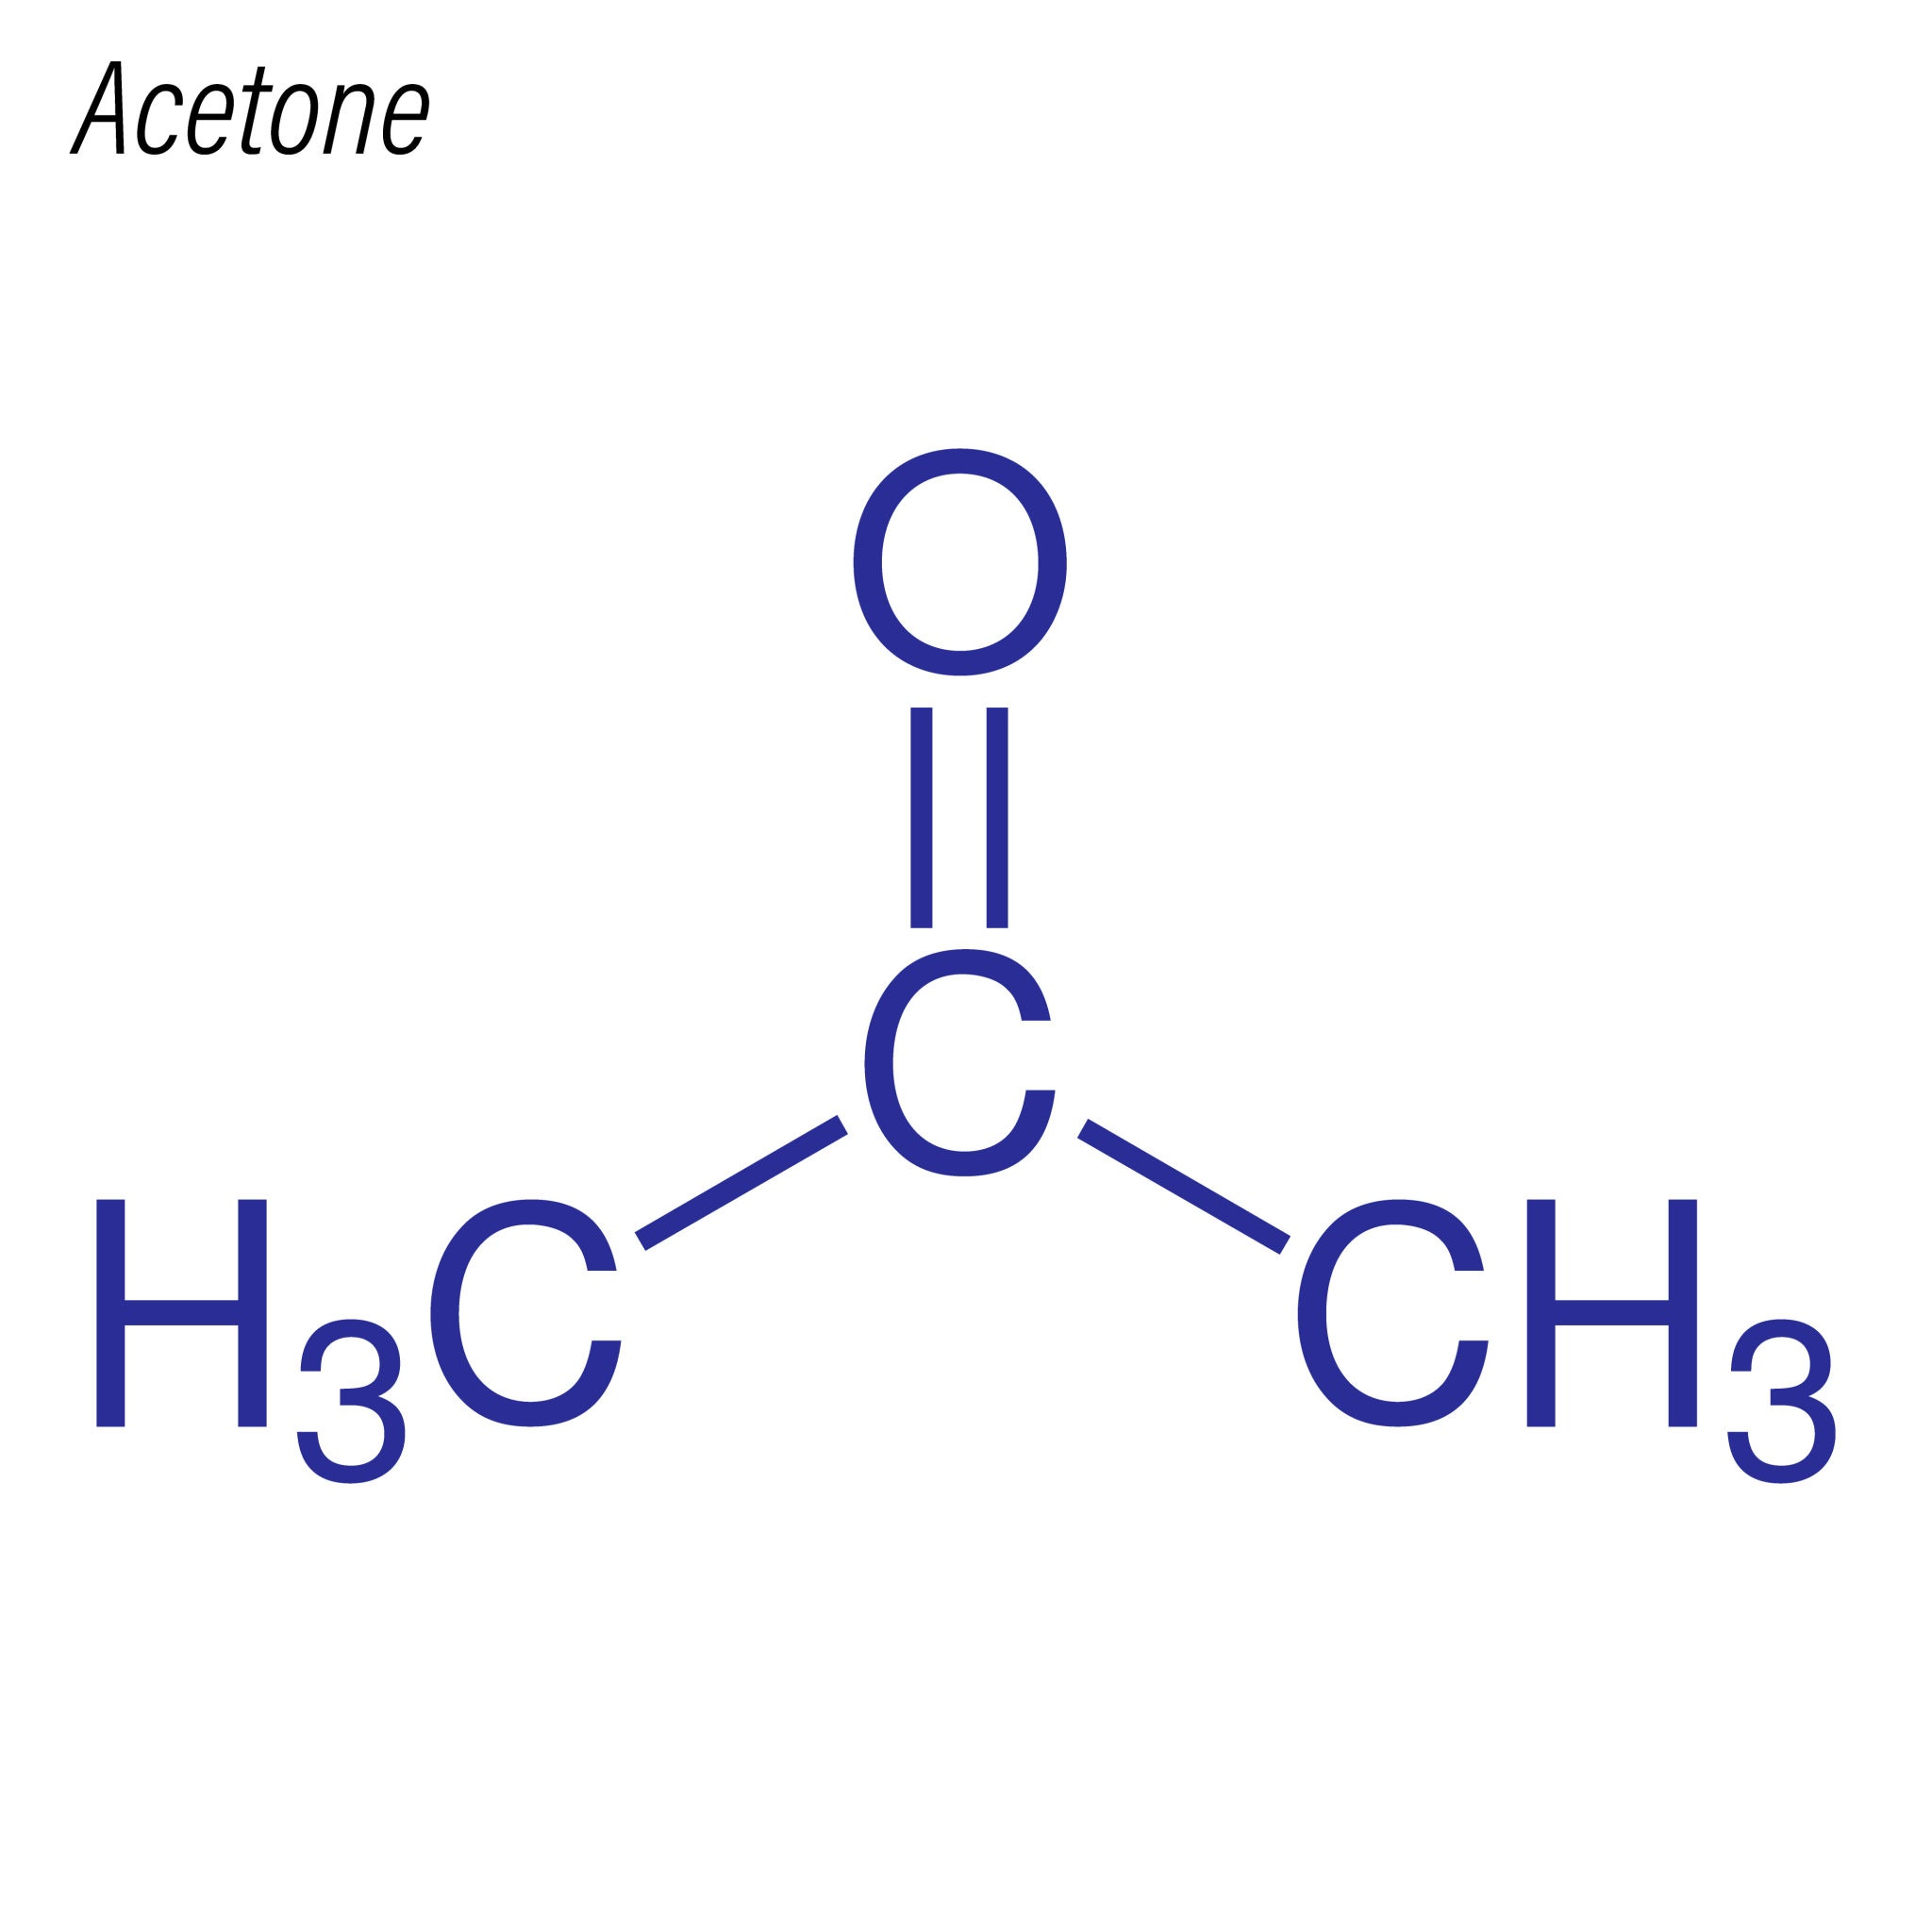
\includegraphics[width=4.5cm,height=4.5cm]{image/tong quan/ctct acetone.jpg}
    \caption{Công thức cấu tạo của acetone}
\end{figure}
Thị trường acetone hiện đang có tốc độ tăng trưởng hàng năm ước tính là 3,4\% từ năm 2023 đến năm 2028. Nhìn chung, thị trường toàn cầu dự kiến sẽ đạt sản lượng 8,6 triệu tấn vào năm 2026. Nhu cầu acetone hằng năm lớn như vậy cũng là hệ quả của nhiều ứng dụng mà acetone đem lại. Acetone được biết đến là một dung môi phân cực không proton có khả năng hoà tan hiệu quả nhiều chất khác nhau, bao gồm chất béo, este cellulose và nhựa. Nó đóng một vai trò quan trọng trong sản xuất thuốc nổ, sợi nhân tạo, dược phẩm, mỹ phẩm, mực in, sơn và vecni. Ngoài ra, acetone còn là tiền chất trong quá trình tổng hợp hóa học của nhiều hợp chất khác.
\begin{figure}[H]
	\centering
    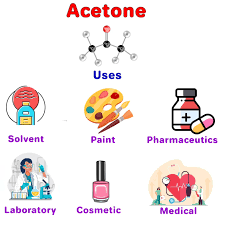
\includegraphics[width=5.75cm,height=5.75cm]{image/tong quan/ung dung acetone.png}
    \caption{Ứng dụng của acetone}
\end{figure}
Acetone là một trong những dung môi công nghiệp ít nguy hiểm nhất, nhưng rất dễ bay hơi và có thể hít phải với số lượng lớn. Nó có thể được hấp thụ vào máu qua phổi và khuếch tán khắp cơ thể. Một lượng nhỏ có thể được hấp thụ qua da. Ở một lượng nhất định khoảng 100 ppm, acetone có thể gây kích ứng mũi, họng, phổi và mắt. Với lượng cao hơn, một số người tiếp xúc với acetone trong không khí ở nồng độ khoảng 250 ppm trong vài giờ đã bị đau đầu và thiếu năng lượng, đồng thời họ cũng bị một số ảnh hưởng nhẹ đến hành vi. Nguy hiểm hơn, khi phơi nhiễm acetone ở nồng độ 12000 ppm hoặc cao hơn tùy thuộc vào thời gian tiếp xúc (từ 2 phút đến 4 giờ) gây đau đầu, choáng váng, chóng mặt, mất thăng bằng và lú lẫn, thậm chí là bất tỉnh. Thêm vào đó, lượng acetone cao trong không khí cũng có một số ảnh hưởng xấu nhất định đến động vật. Theo ACGIH (hội nghị các nhà Vệ sinh Công nghiệp Chính phủ Hoa Kỳ) quy định giới hạn acetone: TWA (Time-Weighted Average) - phơi nhiễm trong 8h - là 250 ppm, STEL (Short-term Exposure Limit) - phơi nhiễm ngắn hạn - là 500 ppm. Thông thường nồng độ acetone trong không khí ở mức độ dưới 8 ppb. Tuy nhiên, trong thời kỳ ngành công nghiệp phát triển như hiện nay thì chất lượng không khí nói chung và lượng acetone trong không khí nói riêng vẫn là một vấn đề đáng được lưu tâm, đặc biệt trong các nhà máy hoá chất.

\subsubsection*{1.2. Quá trình oxi hoá xúc tác}
\phantomsection \addcontentsline{toc}{subsubsection}{\numberline{}1.2. Quá trình oxi hoá xúc tác}

\paragraph*{1.2.1. Các chất xúc tác cho quá trình oxi hoá}
\leavevmode

a) Chất xúc tác kim loại quý

Các kim loại quý được sử dụng rộng rãi làm chất xúc tác cho quá trình xử lí VOCs trong các dòng khí thải nhờ hoạt tính cao trong điều kiện làm việc ở nhiệt độ thấp. Khi được phân tán trên nền chất mang, chúng tạo ra bề mặt hoạt tính cao giúp oxi hoá hầu hết các hợp chất hữu cơ thành carbon dioxide và nước. Các chất xúc tác kim loại quý có đặc tính bền và chịu nhiệt tốt, hiệu suất phản ứng của xúc tác phụ thuộc vào chất mang, phương pháp tổng hợp và nồng độ VOCs. Chất mang thường được sử dụng cho xúc tác kim loại quý là các xúc tác acid rắn như zeolite, zirconium oxide, titanium oxide và silicon oxide với ưu điểm như diện tích bề mặt riêng lớn, tính acid tốt và ổn định nhiệt độ. Các chất mang này không chỉ làm tăng khả năng hấp phụ của vật liệu xúc tác mà còn làm tăng khả năng phân tán của kim loại quý.

Các xúc tác kim loại quý như Pd hay Pt trên nền chất mang thường là $ZrO_2$ hay $TiO_2$ thường là các xúc tác được ưu tiên sử dụng vì hoạt tính rất cao, cho phép xử lý VOCs ở nhiệt độ thấp hơn nhiều so với các hệ xúc tác kim loại chuyển tiếp. Tuy nhiên ứng dụng công nghiệp của xúc tác bởi các kim loại này bị hạn chế vì giá thành cao, khiến chi phí đầu tư ban đầu lớn. Ngoài ra chúng rất nhạy cảm với chất gây nhiễm độc xúc tác, đặc biệt là các hợp chất chứa S, Cl, Pb và silicones dẫn đến cần tái sinh hoặc thay thế xúc tác gây tốn kém. Do vậy chất xúc tác oxide kim loại không quý có giá thành thấp được xem là lựa chọn thay thế tối ưu hơn.

\begin{table}[H]
    \centering
    \begin{tabular}{@{}|
                >{\centering\arraybackslash}m{3.5cm}|    
                >{\centering\arraybackslash}m{2cm}|
                >{\centering\arraybackslash}m{3cm}|
                >{\centering\arraybackslash}m{1.7cm}|
                >{\centering\arraybackslash}m{2cm}|@{}} \hline
        \textbf{Xúc tác} & \textbf{Nồng độ (ppm)} & \textbf{Tốc độ (mL.g$^{-1}$.h$^{-1}$)} & \textbf{$T_{50}$($^o$C)} & \textbf{$T_{90}$($^o$C)}\\ \hline % Tiêu đề
        0.8Pt-G/@Zr & 1000 & 30000 & 187 & 210\\ \hline % Dòng 1
        CeO$_2$-Pt/TiO$_2$ & 1000 & 40000 & 212 & 245\\ \hline % Dòng 2
        Pt$_{0.01}$Mn$_{0.2}$/Ti & 1000 & 30000 & 205 & 209\\ \hline % Dòng 3
        Au-Pd/$\alpha$-MnO$_2$ & 1000 & 40000 & 170 & 180\\ \hline % Dòng 4
        Pt/$\gamma$-Al$_2$O$_3$ & 1000 & 18000 & 121 & 130\\ \hline % Dòng 5
    \end{tabular}
    \caption{\centering Các xúc tác kim loại quý cho quá trình oxi hoá acetone}
\end{table}

b) Chất xúc tác oxide kim loại

Chất xúc tác oxide kim loại hiện là một trong những giải pháp hiệu quả và được nghiên cứu rộng rãi nhất để xử lý hợp chất VOCs bằng phương pháp oxy hóa xúc tác ở nhiệt độ tương đối thấp. Các oxide kim loại chuyển tiếp phổ biến như CeO$_2$, MnO$_x$, Co$_3$O$_4$, CuO, Fe$_2$O$_3$, NiO và đặc biệt là các oxide hỗn hợp như Ce-Mn-O$_x$, Cu-Mn-O$_x$, Ce-Zr-O$_x$ thể hiện hoạt tính vượt trội nhờ khả năng lưu trữ và giải phóng oxy bề mặt tốt. Mặc dù hoạt tính phản ứng không cao như các chất xúc tác kim loại quý, song các chất oxide kim loại vẫn được ưu tiên lựa chọn vì giá thành rẻ, ít bị đầu độc xúc tác, tuổi thọ dài, sự đa dạng về kích thước và hình dạng cũng như khả năng tái sinh tốt.

Cryptomelane ($K_xMn_8O_{16}$, x = 0,2 - 1,0), một (hydr)oxide được biết đến như là một chất hấp phụ hoạt động, chất oxy hoá và xúc tác trong các quá trình địa hóa của các chất môi trường. Cryptomelane là một khoáng chất nanorod được hình thành dựa trên sự ghép nối cạnh và góc chung của 2 đơn vị bát diện $MnO_6$ để xây dựng đường hầm có kích thước 4,6 × 4,6 Å theo cách sắp xếp 2 × 2. Trong $MnO_6$, các nguyên tử oxy chiếm các đỉnh và mangan ở trung tâm của bát diện. Mangan sẽ mang số oxy hoá hỗn hợp trong khoảng 3,6 - 3,8 giữa $Mn^{3+}$ và $Mn^{4+}$. Để cân bằng điện tích sẽ có các ion $K^+$ và nước chứa trong cấu trúc cryptomelane đường hầm (K-OMS-2).
\begin{figure}[H]
	\centering
    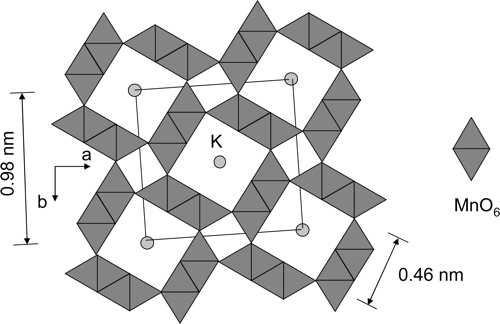
\includegraphics[width=8cm,height=6cm]{image/tong quan/cau truc koms2.png}
    \caption{Cấu trúc của K-OMS-2}
\end{figure}
Việc biến tính oxit mangan bằng các tạp chất kim loại khác nhau ($Me^{n+}$ = $Sn^{4+}$, $Ru^{3+}$, $Ni^{2+}$, $Co^{2+}$, $Fe^{3+}$, $Cu^{2+}$, $V^{5+}$, $Ce^{4+}$,\ldots) cũng có thể tăng cường hoạt tính của oxit mangan đối với các phản ứng oxy hóa. Đối với các cryptomelane được biến tính, do sự hiện diện của $Mn^{2+}$, $Mn^{3+}$ và $Mn^{4+}$ trong cấu trúc cũng như tạo ra các lỗ khuyết oxy làm tinh thể kém bền hơn và tăng khả năng hấp phụ oxy từ pha khí, từ đó tính oxy hóa được cải thiện. Điều này mang lại cho các vật liệu như vậy một lợi thế đáng kể so với nhiều hệ xúc tác khác trong các phản ứng oxy hóa.
\begin{figure}[H]
	\centering
    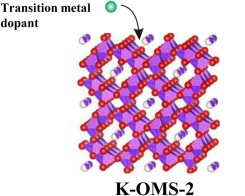
\includegraphics[width=8cm,height=6cm]{image/tong quan/cau truc bien tinh oms-2.png}
    \caption{\centering Cấu trúc của cryptomelane được biến tính kim loại chuyển tiếp}
\end{figure}

Như vậy, các hợp chất cryptomelane (OMS-2) đã thể hiện những tiềm năng đầy hứa hẹn trong việc cải thiện chất lượng không khí. Tuy nhiên, những nghiên cứu liên quan đến OMS-2 vẫn còn đang hạn chế so với ứng dụng mà nó mang lại.

Nickel foam là một loại vật liệu kim loại có cấu trúc không gian ba chiều với độ xốp cực cao (thường > 95\%), được đặc trưng bởi mạng lưới các lỗ rỗng liên thông chặt chẽ. Với diện tích bề mặt riêng lớn và cấu trúc khung xương kim loại có độ dẫn điện tuyệt vời, Nickel foam đóng vai trò là một bệ đỡ lý tưởng cho các quá trình phát triển vật liệu tại chỗ , giúp loại bỏ nhu cầu sử dụng chất kết dính và giảm thiểu điện trở tiếp xúc.
Đặc tính cơ học bền vững cùng khả năng kháng ăn mòn tốt trong nhiều môi trường điện ly giúp vật liệu này duy trì được độ ổn định cấu trúc trong suốt quá trình phản ứng thủy nhiệt và nung ở nhiệt độ cao. Trong các ứng dụng điện hóa và xúc tác, cấu trúc lỗ rỗng của Nickel foam không chỉ tối ưu hóa diện tích tiếp xúc giữa pha hoạt tính và môi trường phản ứng mà còn tạo điều kiện thuận lợi cho sự khuếch tán nhanh chóng của các ion và chất phản ứng xuyên suốt mạng lưới 3D, từ đó nâng cao hiệu suất tổng thể của các hệ điện cực.


\paragraph*{1.2.2. Cơ chế phản ứng xúc tác}
\leavevmode

Trong các phản ứng xúc tác dị thể, chất xúc tác thường ở dạng rắn và các chất phản ứng (tác chất) ở dạng lưu chất (thường là khí hoặc lỏng). Vai trò của chất xúc tác là làm thay đổi vận tốc phản ứng (tăng tốc hoặc kìm hãm) mà không làm thay đổi cân bằng nhiệt động học của hệ. Cơ chế hoạt động của xúc tác rắn thường liên quan đến việc hạ thấp hàng rào năng lượng hoạt hóa, cho phép các phân tử tác chất biến đổi thành sản phẩm dễ dàng hơn so với phản ứng không xúc tác.

\begin{figure}[H]
	\centering
    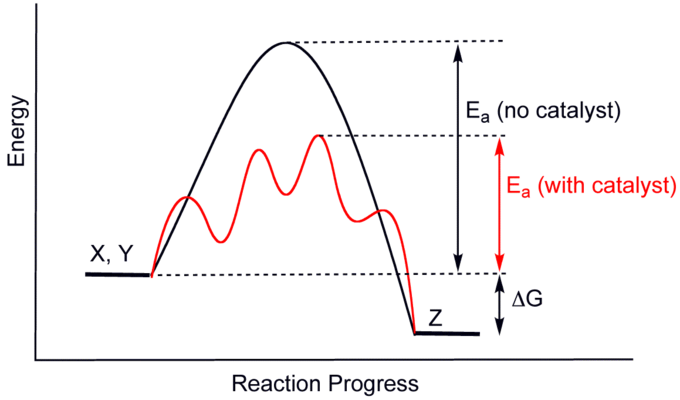
\includegraphics[scale=1.25]{image/tong quan/catalysisscheme.png}
    \caption{Năng lượng hoạt hoá phản ứng khi không có và có xúc tác}
\end{figure}

Để phản ứng xúc tác dị thể xảy ra, điều kiện tiên quyết là các phân tử tác chất phải tiếp xúc và tương tác với bề mặt chất xúc tác. Quá trình biến đổi từ tác chất thành sản phẩm trên xúc tác rắn xốp không xảy ra tức thời mà diễn ra theo một chuỗi 7 giai đoạn nối tiếp nhau \cite{19}. Sự thành công của phản ứng phụ thuộc vào việc vượt qua các trở lực ở từng giai đoạn này:

\begin{figure}[H]
	\centering
    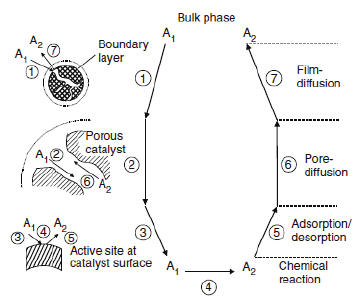
\includegraphics[scale=1]{image/tong quan/ndividual-steps-of-a-simple-heterogeneous-catalytic-fluid-solid-reaction-A-1-A-2.png}
    \caption{Cơ chế 7 giai đoạn phản ứng xúc tác dị thể}
\end{figure}

\begin{enumerate}
    \item Khuếch tán tác chất qua lớp phim: Tác chất từ dòng khí khuếch tán qua lớp phim bao quanh hạt xúc tác để đến bề mặt ngoài của hạt.
    \item Khuếch tán tác chất qua lỗ xốp: Vì diện tích mặt trong lớn hơn nhiều diện tích mặt ngoài nên phần lớn phản ứng xảy ra bên trong hạt, do đó tác chất khuếch tán sâu vào bên trong hạt qua các lỗ xốp.
    \item Hấp phụ (Adsorption): Tại bề mặt bên trong lỗ xốp, các phân tử tác chất kết hợp với các tâm hoạt động (active sites) trên bề mặt xúc tác.
    \item Phản ứng: Đây là bước chuyển hóa hóa học thực sự. Các phân tử đã bị hấp phụ sẽ chuyển hoá ngay trên bề mặt để tạo thành sản phẩm.
    \item Giải hấp (Desorption): Sản phẩm sau khi hình thành sẽ tách rời khỏi tâm hoạt động để trở lại trạng thái tự do trong lỗ xốp.
    \item Khuếch tán sản phẩm qua lỗ xốp: Sản phẩm khuếch tán từ trong lòng lỗ xốp ra ngoài bề mặt hạt.
    \item Khuếch tán sản phẩm qua lớp phim: Sản phẩm khuếch tán qua lớp phim bao quanh hạt để đi vào dòng khí.
\end{enumerate}

Cơ chế phản ứng trên bề mặt được giải thích dựa trên giả thuyết rằng bề mặt xúc tác không đồng nhất hoàn toàn, mà phản ứng chỉ xảy ra tại những vị trí đặc biệt gọi là ``vùng hoạt động'' (active sites). Quá trình này bao gồm việc phân tử gắn vào vùng hoạt động, phản ứng với phân tử bên cạnh (cơ chế hai vùng) hoặc phản ứng trực tiếp, sau đó sản phẩm rời đi để trả lại vùng hoạt động trống.

\subsubsection*{1.3. Phương pháp hấp phụ}
\phantomsection \addcontentsline{toc}{subsubsection}{\numberline{}1.3. Phương pháp hấp phụ}

Hấp phụ là quá trình lắng đọng các phần tử trên bề mặt phân tách (rắn-lỏng, khí-rắn, lỏng-khí, khí-lỏng). Các chất được hấp phụ lên trên bề mặt được gọi là chất bị hấp phụ, và chất nền nơi sự hấp phụ xảy ra gọi là chất hấp phụ. Quá trình chất bị hấp phụ xâm nhập vào các lớp hấp phụ gọi là sự hấp phụ. Quá trình chất bị hấp phụ giải phóng ra khỏi chất hấp phụ gọi là sự giải hấp. Dựa vào lực tương tác giữa các phân tử của chất hấp phụ và chất bị hấp phụ có thể phân ra thành hấp phụ vật lí và hấp phụ hoá học.

Hấp phụ vật lí xảy ra do lực tương tác phân tử Van der Waals khi khoảng cách giữa bề mặt chất hấp phụ và chất bị hấp phụ trở nên gần hơn. Sự liên kết này khá yếu và dễ dàng bị huỷ khi chịu tác động ngoại lực. 

Hấp phụ hoá học xảy ra do sự hình thành các liên kết hoá học giữa bề mặt chất hấp phụ và phân tử chất bị hấp phụ, hình thành các thành phần liên kết trên bề mặt. Nhiệt hình thành của quá trình hấp phụ hoá học khá lớn, do đó liên kết do quá trình này tạo nên rất bền và khó bị phá huỷ.

Trong thực tế, việc phân biệt hấp phụ vật lí và hấp phụ hoá học khá khó vì ranh giới giữa hai loại hấp phụ này là không rõ ràng. Hơn nữa, trong một quá trình hấp phụ có thể xảy ra đồng thời cả hấp phụ vật lí và hấp phụ hoá học.

\begin{figure}[H]
    \centering
    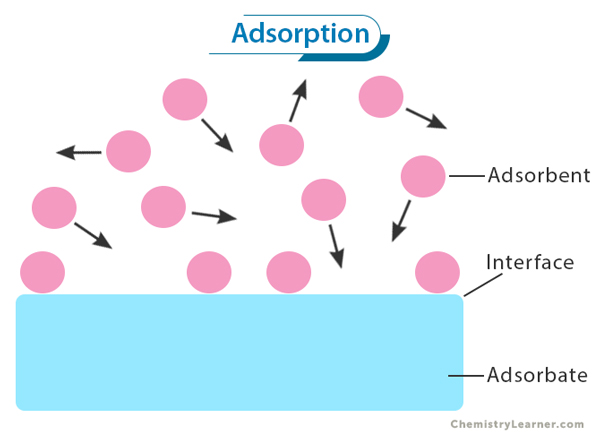
\includegraphics[width=0.8\linewidth]{image/tong quan/mo ta qua trinh hap phu.jpg}
    \caption{Quá trình hấp phụ}
    \label{fig:placeholder}
\end{figure}

\subsubsection*{1.4. Các phương pháp đánh giá}
\phantomsection \addcontentsline{toc}{subsubsection}{\numberline{}1.4. Các phương pháp đánh giá}

\paragraph*{1.4.1. Xray diffraction (XRD)}
\leavevmode

Phương pháp nhiễu xạ tia X (X-ray diffraction-XRD) là kĩ thuật phân tích không phá huỷ, đóng vai trò nền tảng trong khoa học vật liệu để xác định thành phần pha, độ tinh khiết và cấu trúc vi mô các tinh thể rắn (kích thước hạt, độ biến dạng màng). Trong ứng dụng thực tiễn, giá trị cốt lõi của XRD nằm ở khả năng cung cấp ``dấu vân tay'' cấu trúc duy nhất cho từng vật liệu, cho phép các nhà nghiên cứu định danh chính xác các pha tinh thể mà các phương pháp hóa học thông thường không thể phân biệt được. Trong công nghiệp dược phẩm, kỹ thuật này đóng vai trò sinh tử trong việc kiểm soát các dạng thù hình (polymorphs) của hoạt chất, bởi sự thay đổi cấu trúc tinh thể có thể ảnh hưởng trực tiếp đến độ tan và hiệu quả điều trị của thuốc. Đối với lĩnh vực khoa học vật liệu và công nghệ nano, XRD là công cụ đắc lực để xác định kích thước hạt tinh thể, đánh giá độ kết tinh và đo lường ứng suất dư (residual stress) trong kim loại hoặc gốm sau quá trình gia công. Ngoài ra, phương pháp này còn được ứng dụng rộng rãi trong địa chất để phân tích thành phần khoáng vật trong đất đá, cũng như trong công nghiệp bán dẫn để kiểm tra chất lượng các lớp màng mỏng siêu vi, khẳng định vị thế không thể thay thế của XRD trong cả nghiên cứu cơ bản lẫn kiểm soát chất lượng sản xuất. 

Cơ sở của phương pháp dựa trên hiện tượng tán xạ ánh sáng của bề mặt các tinh thể khi các nguyên tử bị kích thích bởi chùm tia X đi qua. Các chùm tia X này sẽ bị nhiễu xạ tạo thành các tia nhiễu xạ với cường độ và hướng khác nhau. Các hướng này bị khống chế bởi bước sóng của bức xạ tới và bởi bản chất của mẫu tinh thể theo định luật Bragg.

Định luật Bragg: Xét một chùm tia X có bước sóng $\lambda$ chiếu tới tinh thể chất rắn dưới góc tới $\theta$. Trong tinh thể, các nguyên tử hay ion được phân bố một cách có đều đặn theo một quy luật xác định, ta giả định các tinh thể sẽ cách nhau những khoảng d đều đặn tạo ra hiện tượng nhiễu xạ tia X. Mối liên hệ giữa sự nhiễu xạ này và khoảng cách d tuân theo công thức sau:

\begin{center}
n$\lambda$=2dsin$\theta$
\end{center}

    Trong đó:
    
        \hspace{1.2cm} d là khoảng cách giữa 2 mặt phẳng tinh thể;
        
        \hspace{1.2cm} $\theta$ là góc tới của chùm tia X so với mặt phẳng tinh thể;
        
        \hspace{1.2cm} n là bậc nhiễu xạ (n là số nguyên);
        
        \hspace{1.2cm} $\lambda$ là bước sóng của tia X.

Phổ XRD cung cấp các thông tin sau:
\begin{itemize}
    \item Vị trí các peak:
    \item Cường độ các peak:
    \item Hình dạng và chiều rộng đỉnh: 
\end{itemize}

Ngoài ra, phương pháp nhiễu xạ tia X còn cho phép xác định kích thước tinh thể dựa theo phương trình Scherrer:

\begin{center}
    $D = \dfrac{k\lambda}{\beta\cos{\theta}}$
\end{center}

    Trong đó:
    
        \hspace{1.2cm} D là kích thước tinh thể;
        
        \hspace{1.2cm} k là hệ số tỉ lệ;
        
        \hspace{1.2cm} $\beta$ là độ bán phổ (tính theo rad).

\begin{figure}[H]
	\centering
    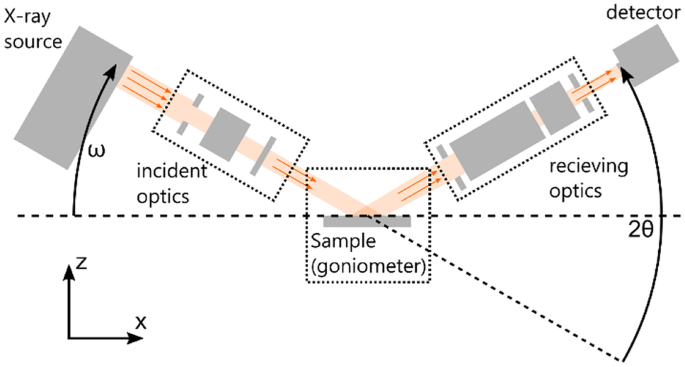
\includegraphics[scale=0.5]{image/danh gia xuc tac/anh minh hoa XRD.png}
    \caption{Nguyên lý hoạt động X-ray Diffraction (XRD)}
\end{figure}

\paragraph*{1.4.2. Scanning electron microscopy (SEM)}
\leavevmode

Kính hiển vi điện tử quét (Scanning Electron Microscopy, viết tắt là SEM) là một trong những phương pháp công cụ phổ biến để phân tích đặc tính hình ảnh và kích thước của các hạt vi mô và hạt nano trên vật thể rắn. Một trong những lý do khiến SEM được dùng nhiều trong phân tích kích thước hạt là nhờ vào độ phóng đại cao. Các phiên bản tiên tiến của loại thiết bị này có thể đạt độ phân giải khoảng 2.5 nm (25 Å).

Thông thường, chùm electron được tạo ra từ đèn dây tóc vonfram hoặc súng phát xạ trường (Field Emission Gun - FEG). Quá trình tăng tốc chùm electron diễn ra thông qua hệ thống cao thế (20 kV), và chùm electron này sẽ hội tụ lại sau khi đi qua các khe khẩu độ và hệ thống thấu kính điện từ. Sau đó, chùm tia sẽ quét lên bề mặt mẫu vật nhờ sự hỗ trợ của các cuộn dây quét. Tương tác giữa electron và các nguyên tử trong mẫu tạo ra các tín hiệu mang thông tin về hình ảnh bề mặt mẫu. Các electron tán xạ ngược (Backscattered electrons) và electron thứ cấp (Secondary electrons) phát ra từ mẫu vật vào môi trường chân không sẽ được thu nhận bởi một đầu dò được đặt ở vị trí thích hợp. Việc tập trung vào một khu vực ở mức độ phóng đại cao (>100 kX) giúp phân tích hình thái bề mặt (topography) của mẫu tốt hơn với độ phân giải không gian tối ưu.

\begin{figure}[H]
	\centering
    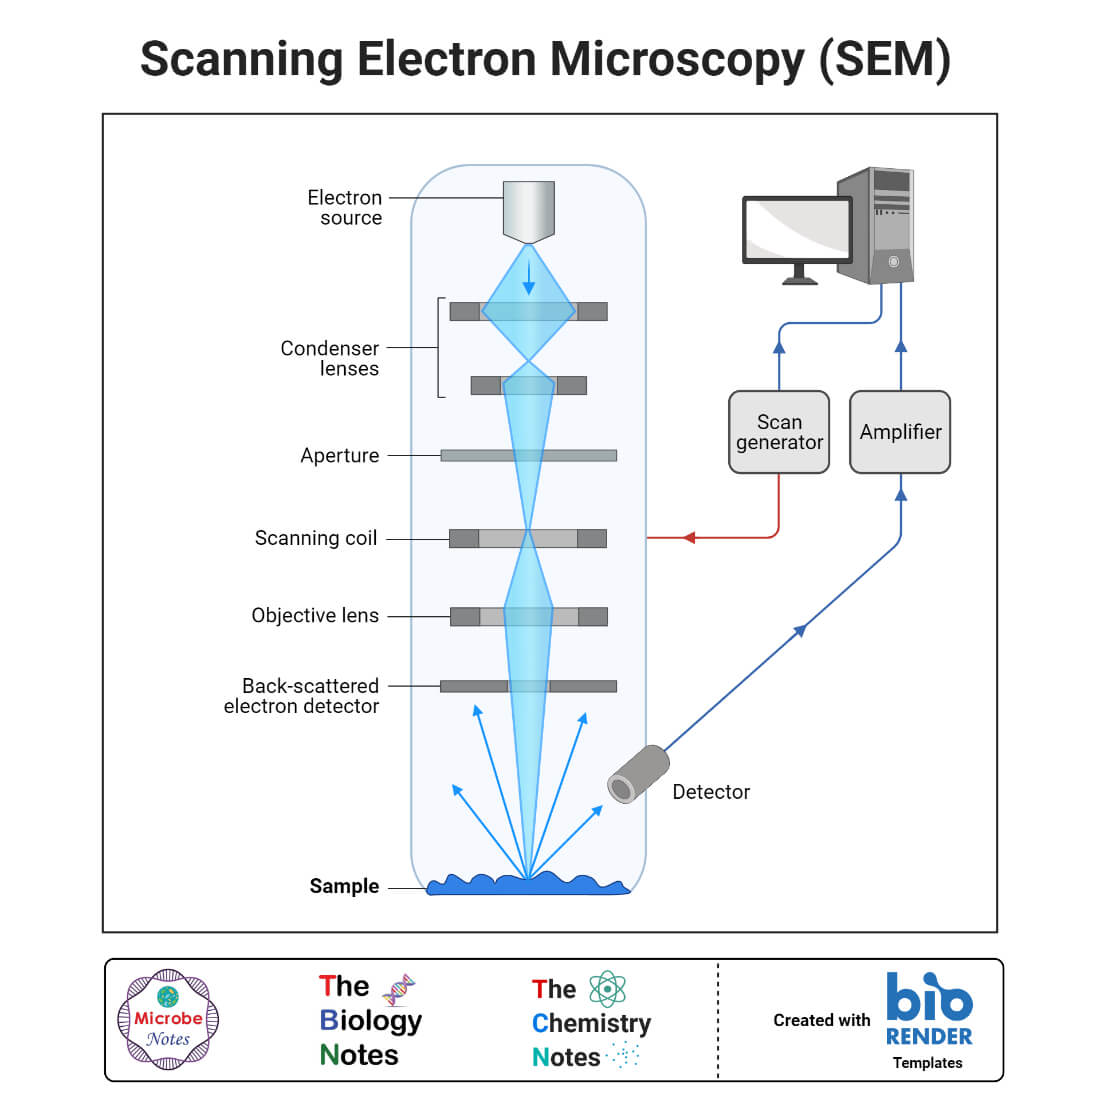
\includegraphics[scale=0.25]{image/danh gia xuc tac/Scanning-Electron-Microscope-SEM.jpeg}
    \caption{Nguyên lý hoạt động Scanning Electron Microscope (SEM)}
\end{figure}

Mặc dù độ phân giải của SEM vẫn không thể so sánh lại với kính hiện vi điện tử truyền qua (TEM) nhưng phương pháp này có ưu điểm hơn trong việc chuẩn bị mẫu dễ dàng, thu thập hình ảnh nhanh chóng cũng như ít chi phí hơn.

\paragraph*{1.4.3.Thermogravimetric analysis (TGA)}
\leavevmode

Phân tích nhiệt trọng lượng (Thermogravimetric Analysis - TGA) là một kỹ thuật phân tích định lượng dùng để theo dõi sự thay đổi khối lượng của mẫu vật theo thời gian hoặc nhiệt độ khi mẫu được gia nhiệt theo một chương trình nhiệt độ được kiểm soát. Phương pháp này cho phép khảo sát các tính chất vật lý và hóa học của vật liệu khi chịu tác động của nhiệt. Trong kỹ thuật hóa học hiện đại, TGA được ứng dụng rộng rãi để xác định độ chuyển hóa, động học phản ứng và cơ chế của bất kỳ quá trình nào có sự thay đổi về khối lượng thông qua các phương pháp đẳng nhiệt hoặc biến thiên nhiệt độ.

Một hệ thống TGA cơ bản bao gồm một cân vi lượng (microbalance) có độ chính xác cao được kết nối với khay chứa mẫu (sample pan) đặt bên trong lò nung (furnace).

\begin{itemize}
    \item Quy trình vận hành: Thiết bị sẽ ghi lại khối lượng mẫu, thời gian và nhiệt độ liên tục. Chương trình nhiệt độ có thể bao gồm quá trình gia nhiệt, làm lạnh, giữ nhiệt độ không đổi (đẳng nhiệt) hoặc kết hợp các quá trình này.
    \item Môi trường khí: Mẫu được nung trong môi trường khí được kiểm soát (purge gas) chảy qua mẫu với lưu lượng từ 20-200 mL/phút. Khí này có thể là khí trơ (như Argon, Helium, Nitrogen) để ngăn phản ứng, hoặc khí oxy hóa (như không khí, Oxy) để đốt cháy mẫu hữu cơ và oxy hóa kim loại, hoặc khí khử.
    \item Cơ chế thay đổi khối lượng:
    \begin{itemize}
        \item Khối lượng mẫu giảm khi xảy ra sự phân hủy, bay hơi các hợp chất dễ bay hơi, hoặc trạng thái oxy hóa giảm.
        \item Khối lượng mẫu tăng trong môi trường phản ứng (ví dụ có $O_2$), nơi các kim loại chuyển tiếp có thể bị oxy hóa.
        \item Tuy nhiên, TGA không thể phát hiện các quá trình chuyển pha, biến đổi đa hình hoặc các phản ứng không gây ra sự thay đổi khối lượng.
    \end{itemize}
\end{itemize}

\begin{figure}[H]
	\centering
    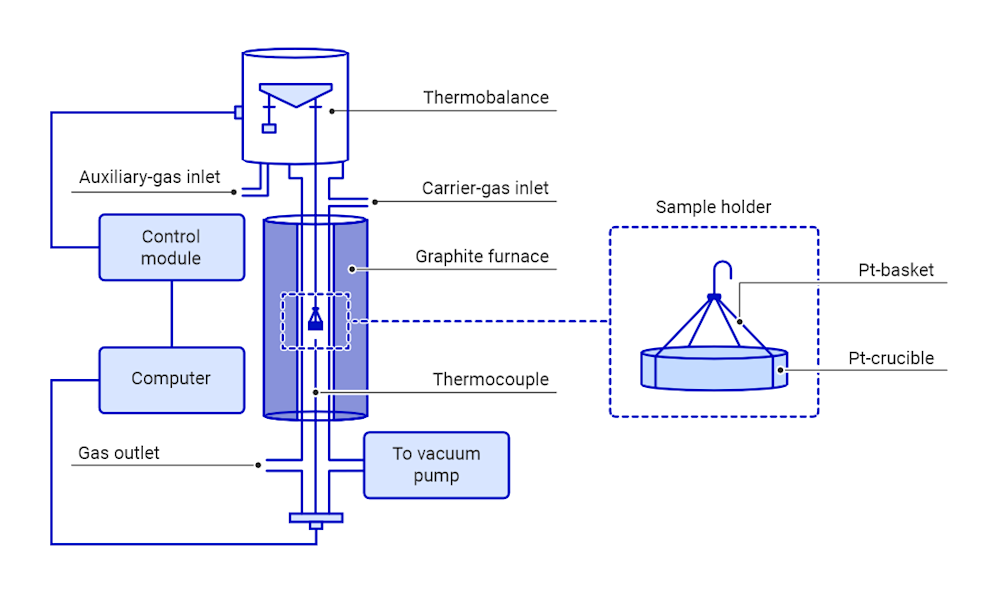
\includegraphics[scale=0.375]{image/danh gia xuc tac/TGA_diagram_3.png}
    \caption{Nguyên lý hoạt động Thermogravimetric Analysis (TGA)}
\end{figure}

Các cấu hình thiết bị thường gặp bao gồm nạp mẫu từ trên xuống (top-loading), treo mẫu từ dưới lên (bottom-loading/hang-down), hoặc nạp ngang (side-loading).

Kết quả của phép đo TGA được biểu diễn dưới dạng đường cong nhiệt (thermogram) – đồ thị biểu diễn sự thay đổi khối lượng (hoặc phần trăm khối lượng) theo nhiệt độ hoặc thời gian. Một biểu đồ TGA điển hình thường chia thành các giai đoạn phân hủy theo nhiệt độ:

\begin{itemize}
    \item Dưới $150^oC$: Sự giảm khối lượng thường do nước hấp phụ vật lý, các hợp chất dễ bay hơi có khối lượng phân tử thấp hoặc dung môi bay hơi.
    \item Từ $150^oC$ - $250^oC$: Sự mất khối lượng liên quan đến nước hấp phụ hóa học, các chất phụ gia và các sản phẩm phân hủy dễ bay hơi.
    \item Trên $250^oC$: Các hợp chất bắt đầu phân hủy mạnh (xác định bởi nhiệt độ bắt đầu - onset và kết thúc - endset).
    \item Phần còn lại: Sau khi kết thúc quá trình gia nhiệt, phần vật liệu còn lại thường là tro vô cơ không bay hơi hoặc kim loại.
\end{itemize}

Để phân tích chính xác hơn các điểm uốn và tách biệt các quá trình phản ứng chồng chéo nhau, người ta thường sử dụng đường đạo hàm bậc một và đạo hàm bậc hai của đường cong khối lượng.

Biểu đồ nhiệt cung cấp thông tin quan trọng về độ bền nhiệt, độ bền oxy hóa, thành phần đa cấu tử, tuổi thọ sản phẩm, động học phân hủy, cũng như hàm lượng ẩm và chất dễ bay hơi của vật liệu. Ngoài ra, TGA còn có thể kết hợp với các thiết bị phân tích khí (như GC, MS, FTIR) để định danh chính xác các khí thoát ra trong quá trình nung.

\paragraph*{1.4.4. Phân tích nguyên tố}
\leavevmode

Quang phổ hấp thu nguyên tử (Atomic Absorption Spectroscopy - AAS) là một kỹ thuật phân tích định lượng được sử dụng rộng rãi để xác định nồng độ các nguyên tố kim loại và á kim trong mẫu vật. Phương pháp này được phát triển lần đầu tiên vào năm 1952 bởi Sir Alan Walsh tại CSIRO (Úc) và chính thức thương mại hóa vào những năm 1960. Đến nay, AAS vẫn là tiêu chuẩn trong các phòng thí nghiệm nhờ độ tin cậy và tính đơn giản.

AAS hoạt động dựa trên nguyên lý sự hấp thu năng lượng ánh sáng của các nguyên tử tự do. Ở điều kiện bình thường, các nguyên tử kim loại tồn tại ở trạng thái năng lượng thấp nhất, được gọi là ``trạng thái cơ bản''. Dưới tác dụng của năng lượng (ở đây là ánh sáng), electron trạng thái cơ bản sẽ hấp thu để di chuyển đến trạng thái năng lượng cao hơn, được gọi là ``trạng thái kích thích''. Dựa theo nguyên tắc này, chùm sáng đi qua đám mây nguyên tử càng bị yếu đi bao nhiêu, chứng tỏ số lượng nguyên tử trong mẫu càng nhiều bấy nhiêu.

Để hiện thực hóa nguyên lý trên, hệ thống máy AAS bao gồm 4 bộ phận chính hoạt động theo quy trình sau:
\begin{itemize}
    \item Nguồn phát tia bức xạ: Đèn Cathode rỗng (Hollow Cathode Lamp - HCL) là nguồn sáng phổ biến nhất được sử dụng trong AAS. Đèn Cathode rỗng có cấu tạo chứa khí trơ (Neon hoặc Argon) và một cathode kim loại, được phủ nguyên tố cần nghiên cứu, được đặt đối diện với anode. Khi có dòng điện, khí trơ bị ion hóa và bắn phá vào cathode, làm bật các nguyên tử kim loại ra. Các va chạm tiếp theo giữa các nguyên tử kim loại diễn ra, đưa chúng lên trạng thái kích thích. Khi các nguyên tử đó trở về trạng thái cơ bản sẽ phát xạ ánh sáng có bước sóng đặc trưng cho nguyên tố đó.
    \item Hệ thống hóa hơi mẫu: Đây là bộ phận quan trọng nhất, có nhiệm vụ chuyển mẫu từ dạng dung dịch sang dạng nguyên tử tự do (hơi). Đầu đốt lửa là nguồn nguyên tử hoá phổ biến nhất đối với AAS, tuy nhiên vẫn có những lựa chọn thay thế khác tuỳ vào mục đích cụ thể như lò graphite hay máy tạo hydride. Có hai hỗn hợp khí phổ biến được dùng làm nhiên liệu cho ngọn lửa: không khí-axetilen và nitơ oxit-axetilen. Với việc tạo ra ngọn lửa ở nhiệt độ khoảng $2300^oC$, không khí-axetilen phù hợp với hầu hết các nguyên tố.Còn ở khoảng $2700^oC$, ngọn lửa nitơ oxit-axetilen tạo ra môi trường khử mạnh hơn, phù hợp với các nguyên tố dễ tạo oxit. Có 4 giai đoạn chính diễn ra trong đầu đốt lửa AAS, đó là
    \begin{itemize}
        \item Khử dung môi. Dung môi bị bay hơi hết, để lại các hạt mẫu vô cùng nhỏ (hạt nano) ở dạng khô.
        \item Hóa hơi. Các hạt mẫu được chuyển sang thể khí.
        \item Nguyên tử hóa. Đây là giai đoạn then chốt để tạo ra tập hợp các nguyên tử tự do ở trạng thái cơ bản. Các nguyên tử ở trạng thái cơ bản này chính là mục tiêu để máy AAS thực hiện phân tích.
        \item Ion hóa. Một số nguyên tử tự do sẽ bị chuyển đổi thành các ion.
    \end{itemize}
    Trong quy trình AAS chuẩn, chúng ta mong muốn giai đoạn 1, 2, 3 xảy ra hoàn toàn, nhưng lại muốn hạn chế giai đoạn 4 do máy AAS chỉ đo được nguyên tử trung hòa (vì đèn Cathode rỗng phát ra năng lượng tương ứng với nguyên tử trung hoà).
    \item Bộ đơn sắc: Sau khi chùm sáng đi qua đám mây nguyên tử, nó sẽ đi vào bộ đơn sắc. Thông thường, đèn cathod rỗng phát ra nhiều vạch phát xạ hẹp. Bộ phận này dùng cách tử (optical grating) để cô lập một vạch phát xạ cộng hưởng duy nhất cần đo. Tất cả các bước sóng khác sẽ nằm bên trong máy đơn sắc.
    \item Đầu dò: Đầu dò được sử dụng nhiều nhất trong máy quang phổ hấp thụ nguyên tử là ống nhân quang (photomultiplier tube - PMT). PMT chuyển đổi ánh sáng tới thành tín hiệu điện, cho phép đo cường độ ánh sáng. Ánh sáng từ khe thoát của máy đơn sắc đi vào PMT và chiếu vào một điốt quang, tạo ra tín hiệu điện. Từ cường độ ánh sáng, phương pháp định lượng tuân theo định luật Lambert-Beer:
    
    \begin{center}
        $A=-\log(\dfrac{I}{I_0})=\epsilon lC$
    \end{center}

    Trong đó:
    
        \hspace{1.2cm} $A$: Độ hấp thụ quang;
        
        \hspace{1.2cm} $\epsilon$: Hệ số hấp thụ mol;
        
        \hspace{1.2cm} $l$: Chiều dài đường đi. Đối với AAS ngọn lửa, thường là chiều dài đầu đốt ngọn lửa;
        
        \hspace{1.2cm} $C$: Nồng độ nguyên tố cần phân tích.
\end{itemize}

\begin{figure}[H]
	\centering
    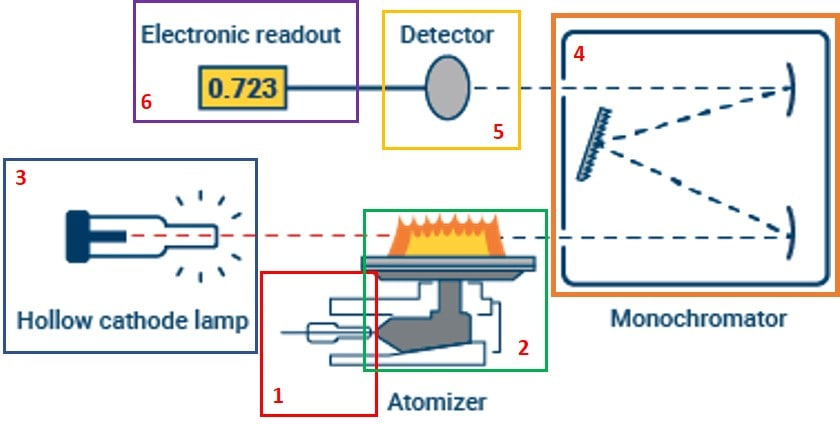
\includegraphics[scale=1]{image/danh gia xuc tac/quy trinh Atomic absorption spectroscopy.jpg}
    \caption{Quy trình quang phổ hấp thụ nguyên tử ngọn lửa đơn giản}
\end{figure}

AAS là phương pháp phân tích thiết yếu trong các lĩnh vực môi trường, thực phẩm và y tế nhờ khả năng xác định kim loại với độ chính xác cao và quy trình đã được chuẩn hóa toàn cầu. Việc lựa chọn kỹ thuật hóa hơi (ngọn lửa hay lò graphite) phụ thuộc vào yêu cầu về độ nhạy và nền mẫu phân tích.

\paragraph*{1.4.5. Xác định trạng thái oxy hoá trung bình của Mangan}
\leavevmode

\paragraph*{1.4.5.1. Nguyên tắc}
\leavevmode

Trong môi trường HCl khoảng 2 -- 3M, Mn hoá trị cao trong mẫu oxide (Mn(III) hay Mn(IV)) sẽ oxy hoá KI thành $I_2$ và Mn(II). Lượng $I_2$ tạo thành được chuẩn độ bằng $Na_2S_2O_3$ với chất chỉ thị là hồ tinh bột. Số oxi hoá Mn được tính theo công thức:

\begin{center}
    $Mn-AOS=\dfrac{C_{Na_2S_2O_3}[V_{Na_2S_2O_3 \text{(mẫu)}}-V_{Na_2S_2O_3 \text{(trắng)}}] \times 10^{-3}}{m_{\text{mẫu}}(\dfrac{\%Mn}{100 \times 54,94})}+2$
\end{center}

Trong đó:
    
        \hspace{1.2cm} $C_{Na_2S_2O_3}$ là nồng độ đương lượng của dung dịch $Na_2S_2O_3$ lúc chuẩn độ;
        
        \hspace{1.2cm} $V_{Na_2S_2O_3 \text{(mẫu)}}$ là thể tích dung dịch $Na_2S_2O_3$ khi chuẩn độ mẫu OMS;
        
        \hspace{1.2cm} $V_{Na_2S_2O_3 \text{(trắng)}}$ là thể tích dung dịch $Na_2S_2O_3$ khi chuẩn độ mẫu trắng;

        \hspace{1.2cm} $m_{\text{mẫu}}$ là khối lượng mẫu khi tiến hành thí nghiệm;

        \hspace{1.2cm} \%Mn là \%Mn trong mẫu đã được xác định từ trước.

\paragraph*{1.4.5.2. Nguyên liệu}
\leavevmode

\begin{table}[H]
    \centering
    \begin{tabular}{@{}|c|p{4.5cm}|p{3cm}|c|c|@{}} \hline
        \textbf{STT} & \centering \textbf{Hoá chất} & \centering \textbf{Công thức hoá học} & \textbf{Trạng thái} & \textbf{Nguồn gốc}\\ \hline
        1 & \centering Sodium thiosulfate pentanhydrate & \centering $Na_2S_2O_3.5H_2O$ & Rắn & Trung Quốc\\ \hline
        2 & \centering Potassium dichromate & \centering $K_2Cr_2O_7$ & Rắn & Trung Quốc\\ \hline
        3 & \centering Potassium iodide & \centering $KI$ & Rắn & Trung Quốc\\ \hline
        4 & \centering Hydrochloric acid & \centering $HCl$ & Lỏng & Trung Quốc\\ \hline
        5 & \centering Starch solute & \centering $(C_6H_{10}O_5)_n$ & Rắn & Trung Quốc\\ \hline
    \end{tabular}
    \caption{\centering Hoá chất dùng trong quá trình xác định trạng thái oxy hoá trung bình của Mangan}
\end{table}

\paragraph*{1.4.5.3. Chuẩn bị}
\leavevmode

a) Chuẩn bị dung dịch sodium thiosulfate

Dung dịch $Na_2S_2O_3$ 0,1N thu được khi hòa tan 12,5g $Na_2S_2O_3.5H_2O$ trong 500 mL nước cất đun sôi để nguội. Bảo quản dung dịch trong tối ở chỗ lạnh và tránh hơi acid.

b) Chuẩn bị dung dịch potassium dichromate

Hòa tan 0,4904g $K_2Cr_2O_7$ đã được sấy khô từ trước ở $100^oC$ trong 2h vào 100 mL nước cất, ta được dung dịch $K_2Cr_2O_7$ 0,1N.

c) Chuẩn bị dung dịch hydrochloric acid

Cho 100 mL $HCl$ đậm đặc 36\% với 100 mL nước cất thu được dung dịch $HCl$ 6M.

d) Chỉ thị hồ tinh bột

Khuấy 1g tinh bột tan được với nước cất (starch solute) rồi rót vào 80 mL nước cất đang sôi. Khuấy đến tan rồi để nguội. Trữ trong tủ lạnh được 1 tuần, nếu không trữ lạnh thì phải pha mới ngay trong ngày tiến hành thí nghiệm.

\paragraph*{1.4.5.4. Quy trình}
\leavevmode

a) Xác định nồng độ của $Na_2S_2O_3$

Hút chính xác 5 mL (dùng pipet bầu) dung dịch $K_2Cr_2O_7$ 0.1 N vào erlen 250 mL, thêm 50 mL nước + 1g KI và 5 mL HCl 6M. Lắc đều và để yên trong 30 giây. Cho $Na_2S_2O_3$ vào buret và chỉnh về vạch 0 mL. Chuẩn độ dung dịch trong erlen bằng $Na_2S_2O_3$ đến khi màu nâu chuyển sang màu vàng nhạt, thêm vài giọt hồ tinh bột. Lúc này dung dịch trong erlen chuyển sang màu xanh đen. Tiếp tục chuẩn độ bằng $Na_2S_2O_3$ đến khi mất màu hoàn toàn. Ghi nhận thể tích dung dịch $V_{Na_2S_2O_3}$ sử dụng và tính nồng độ $Na_2S_2O_3$ theo công thức:

\begin{center}
    $C_{Na_2S_2O_3}=\dfrac{0,5 \times 1}{V_{Na_2S_2O_3}}$
\end{center}

b) Xác định số oxy hoá trung bình của mangan

Cân chính xác 0,05g OMS vào becher 100 mL, dùng bình xịt nước cất chuyển toàn bộ bột đen vào erlen sạch. Cho khoảng 1g KI vào erlen, lắc đều rồi đậy bình bằng nút nhám. Tiếp theo, hút 15 mL HCl 6 M vào becher 100 mL chứa mẫu lúc đầu, xoay đều hòa tan hết những vết đen còn dính trong cốc rồi chuyển hết vào erlen. Tổng thể tích vào khoảng 50 -- 60 mL dung dịch. Lắc đều và đậy erlen bằng nút nhám rồi đánh siêu âm đến khi tan hết. Dùng ít nước cất để lôi kéo các hạt đen bám trên thành bình erlen vào dung dịch. Đậy bình và để yên trong 15 phút để kết tủa hoàn toàn. Sau 15 phút, mở nắp rồi tiến hành chuẩn độ dung dịch màu nâu trong erlen bằng $Na_2S_2O_3$ đến khi chuyển thành màu vàng nhạt. Thêm hồ tinh bột và tiếp tục chuẩn độ đến khi mất màu. Ghi nhận $V_{Na_2S_2O_3 \text{(mẫu)}}$ từ buret. Tiến hành phân tích ít nhất 3 lần để lấy kết quả trung bình.

Thêm 15 mL HCl 6 M và 50 -- 60 mL nước cất vào erlen rồi cho vào 1g KI. Lắc đều và đậy erlen bằng nút nhám, đánh siêu âm cho tan hết (khoảng 2 phút). Đậy bình và để yên trong 15 phút. Sau 15 phút, thêm hồ tinh bột, nếu dung dịch trong erlen có màu xanh đen hoặc màu xanh thì tiến hành chuẩn độ bằng $Na_2S_2O_3$ đến khi mất màu. Ghi nhận $V_{Na_2S_2O_3 \text{(trắng)}}$ từ buret.

Từ đó, ta xác định được hóa trị của Mn theo công thức đã đề cập ở phần 3.5.1.


\subsection*{2. Quy trình}
\phantomsection \addcontentsline{toc}{subsection}{\bfseries \numberline{}2. Quy trình}
\setcounter{section}{2}
\setcounter{figure}{0}
\setcounter{table}{0}

\subsubsection*{2.1. Quy trình tiền xử lí Nickel foam}
\phantomsection \addcontentsline{toc}{subsubsection}{\numberline{}2.1. Quy trình tiền xử lí Nickel foam}

Nickel foam được rửa siêu âm trong dung dịch HCl nồng độ 1mol/L trong 30 phút, sau đó được rửa siêu âm trong nước cất 5 phút và rửa siêu âm trong dung dịch etanol 5 phút để loại bỏ oxit nickel và tạp chất trên bề mặt nickel foam. Sau khi sấy tại 60 độ C trong 3 giờ, nickel foam được cắt thành các miếng với kích thước 4.5 cm*6 cm*1 mm.

\subsubsection*{2.2. Quy trình tổng hợp xúc tác}
\phantomsection \addcontentsline{toc}{subsubsection}{\numberline{}2.2. Quy trình tổng hợp xúc tác}

Xúc tác được tổng hợp bằng phương pháp thuỷ nhiệt trong autoclave dưới điều kiện áp suất và nhiệt độ cao. Hoà tan KMnO4 và CuCl2.2H2O trong nước đến 100ml dung dịch với tỉ lệ Mn/Cu ở các giá trị 4/1, 2/1, 1/1 và 1/0 với tổng nồng độ mol tác chất là 1mol/L. Sau đó, một mẫu nickel foam đã được tiền xử lí được ngâm hoàn toàn trong dung dịch đã pha và được đưa vào autoclave có vỏ ngoài là thép không gỉ và lớp trong là Teflon. Sau khi thuỷ nhiệt tại điều kiện nhiệt độ 120 độ C trong 6 giờ.

\subsubsection*{2.4. Xác định nồng độ acetone đầu vào hệ thống khí}
\phantomsection \addcontentsline{toc}{subsubsection}{\numberline{}2.4. Xác định nồng độ acetone đầu vào hệ thống khí}
Trong hoá học phân tích, lượng hơi acetone trong hệ thống khí có thể được định lượng bằng thuốc thử dung dịch sodium nitroprusside.

Sodium nitroprusside (SPN) có công thức hóa học là $Na_2[Fe(CN)_5NO]$.
Đặc tính nổi bật của SPN là khả năng phản ứng với các carbon nucleophile, đặc biệt là nhóm ketone và các hợp chất carbonyl chứa nguyên tử hydro linh động (có tính acid). Trong đó, tương tác hóa học giữa SPN và acetone là mô hình phản ứng được nghiên cứu đầy đủ và rộng rãi nhất \cite{16}. Cơ chế phản ứng của thuốc thử sodium nitroprusside với acetone:

\begin{center}
    $CH_3COCH_3 + OH^- \rightarrow CH_3COCH_2^- + H_2O$
\end{center}

\hspace{3cm} Acetone \hspace{1.75cm} Anion của acetone

\begin{center}
    $[Fe(CN)_5NO]^{2-} + CH_3COCH_2^- \rightarrow [Fe(CN)_5NOCH_3COCH_2]^{3-}$
\end{center}

\hspace{0.25cm} Nitroprusside ion \hspace{0.25cm} Anion của acetone \hspace{0.25cm} tạo phức màu đỏ

Xác định màu sắc:

Quy trình thử nghiệm được tiến hành bằng cách phản ứng acetone trong môi trường chứa muối ammonium hoặc acetic acid, sau đó kiềm hóa bằng dung dịch ammonia để phát triển màu \cite{17}. Các nghiên cứu tối ưu hóa điều kiện thí nghiệm cho thấy:

Về nồng độ thuốc thử, Sodium nitroprusside được sử dụng ở nồng độ $1\%\ \text{w/v}$. Các kết quả cho thấy việc sử dụng nồng độ cao hơn ($> 2\%\ \text{w/v}$) dẫn đến hiện tượng dung dịch bị đục, ảnh hưởng đến độ chính xác của phép đo. Đối với nguồn cung cấp ion ammonium, Ammonium acetate (nồng độ $25\%\ \text{w/v}$) được ưu tiên lựa chọn thay thế cho acetic acid nhằm đạt được độ sáng màu tối ưu. Mặc dù độ sáng màu tỉ lệ thuận với nồng độ muối ammonium, nhưng thực nghiệm chỉ ra rằng ở nồng độ quá cao, độ sáng trở nên nhạy cảm với những biến đổi nhỏ của nồng độ muối, gây khó khăn cho việc kiểm soát. Do đó, nồng độ $25\%\ \text{w/v}$ là mức phù hợp nhất. Còn môi trường kiềm, dung dịch Ammonia ($50\%\ \text{v/v}$) được xác định là tác nhân kiềm hóa hiệu quả nhất. So với sodium carbonate hay hydroxide, ammonia không chỉ tạo ra màu tím đặc trưng rõ nét hơn mà còn đảm bảo sự cân bằng tốt giữa tốc độ phát triển màu và độ bền của màu sắc tạo thành.

\paragraph*{2.4.1. Nguyên liệu}
\leavevmode

\begin{table}[H]
    \centering
    \begin{tabular}{@{}|c|p{3cm}|p{4.75cm}|c|c|@{}} \hline
        \textbf{STT} & \centering \textbf{Hoá chất} & \centering \textbf{Công thức hoá học} & \textbf{Trạng thái} & \textbf{Nguồn gốc}\\ \hline
        1 & \centering Acetone & \centering $CH_3COCH_3$ & Lỏng & Trung Quốc\\ \hline
        2 & \centering Sodium nitroprusside dihydrate & \centering $Na_2[Fe(CN)_5NO].2H_2O$ & Rắn & Trung Quốc\\ \hline
        3 & \centering Ammonium acetate & \centering $CH_3COONH_4$ & Rắn & Trung Quốc\\ \hline
        4 & \centering Ammonia & \centering $NH_4OH$ & Lỏng & Trung Quốc\\ \hline
        5 & \centering Khí $N_2$ nguyên chất & \centering $N_2$ & Khí & Việt Nam\\ \hline
        6 & \centering Khí $O_2$ nguyên chất & \centering $O_2$ & Khí & Việt Nam\\ \hline
    \end{tabular}
    \caption{\centering Hóa chất sử dụng trong quá trình xác định nồng độ acetone ban đầu}
\end{table}

\paragraph*{2.4.2. Chuẩn bị thuốc thử}
\leavevmode

a) Chuẩn bị dung dịch sodium nitroprusside

Hòa tan 1,00g sodium nitroprusside và 25,0 g ammonium acetate trong nước và định mức đến 100 mL. Bảo quản trong bóng tối, dưới 27°C, và sử dụng trong khoảng thời gian từ 16 đến 24 giờ sau khi pha chế.

b) Chuẩn bị dung dịch ammonia

Pha loãng 25 mL dung dịch ammonia đậm đặc (trọng lượng riêng 0,88) thành 50 mL với nước cất. Bảo quản trong chai nắp kín và pha chế mới hàng ngày.

c) Chuẩn bị thuốc thử

Thuốc thử sẽ gồm 5 mL dung dịch ammonia đã chuẩn bị và 70 mL dung dịch sodium nitroprusside.

\paragraph*{2.4.3. Dựng đường chuẩn}
\leavevmode

a) Chuẩn bị dung dịch chuẩn làm việc acetone

Lấy x mL dung dịch acetone nguyên chất rồi định mức thành 100 mL, với x cụ thể được thể hiện trong bảng 2.5.

\begin{table}[H]
    \centering
    \begin{tabular}{@{}|p{5cm}|p{5cm}|c|@{}} \hline
        \centering \textbf{Nồng độ dung dịch chuẩn làm việc (mg/mL)} & \centering \textbf{Thể tích dung dịch nguyên chất (mL)} & \textbf{Tổng thể tích (mL)}\\ \hline
        \centering 1,96175 & \centering 0,25 & 100\\ \hline
        \centering 3,1388 & \centering 0,4 & 100\\ \hline
        \centering 4,7082 & \centering 0,6 & 100\\ \hline
        \centering 5,88525 & \centering 0,75 & 100\\ \hline
        \centering 7,0623 & \centering 0,9 & 100\\ \hline
        \centering 7,847 & \centering 1 & 100\\ \hline
        \centering 9,80875 & \centering 1,25 & 100\\ \hline
        \centering 11,7705 & \centering 1,5 & 100\\ \hline
    \end{tabular}
    \caption{\centering Nồng độ dung dịch chuẩn làm việc acetone}
\end{table}

b) Xây dựng đường chuẩn thể hiện mối quan hệ giữa nồng độ acetone và độ hấp thu

Xây dựng đường chuẩn thể hiện mối quan hệ giữa nồng độ acetone và độ hấp thu theo các nồng độ acetone cho trước. Việc xây dựng đường chuẩn này dựa trên khả năng tuyến tính của các điểm nồng độ nằm trong khoảng tuyến tính.

Cho 5 mL dung dịch chuẩn làm việc acetone đã pha với nồng độ xác định vào 5 mL thuốc thử đã chuẩn bị. Đợi phản ứng trong 10 phút rồi sử dụng máy quang phổ UV-Vis để đo độ hấp thu ở bước sóng 550 nm. Kết quả được thể hiện ở bảng 2.6.

\begin{table}[H]
    \centering
    \begin{tabular}{@{}|p{5cm}|c|@{}} \hline
        \centering \textbf{Nồng độ dung dịch sau pha trộn (mg/mL)} & \textbf{Độ hấp thu A}\\ \hline
        \centering 0,980875 & 0,103\\ \hline
        \centering 1,5694 & 0,191\\ \hline
        \centering 2,3541 & 0,329\\ \hline
        \centering 2,942625 & 0,426\\ \hline
        \centering 3,53115 & 0,529\\ \hline
        \centering 3,9235 & 0,587\\ \hline
        \centering 4,904375 & 0,665\\ \hline
        \centering 5,88525 & 0,785\\ \hline
    \end{tabular}
    \caption{\centering Độ hấp thu đối với mỗi dung dịch chuẩn làm việc Acetone}
\end{table}

Từ đó, ta xây dựng được phương trình đường chuẩn là

\begin{center}
    $y=0,141x-0,00806$

    với $R^2=0,9829$
\end{center}

Trong đó:
    
    \hspace{1.2cm} $x$: Tương ứng nồng độ của acetone (mg/mL);
        
    \hspace{1.2cm} $y$: Tương ứng độ hấp thu của dung dịch.

\begin{figure}[H]
	\centering
    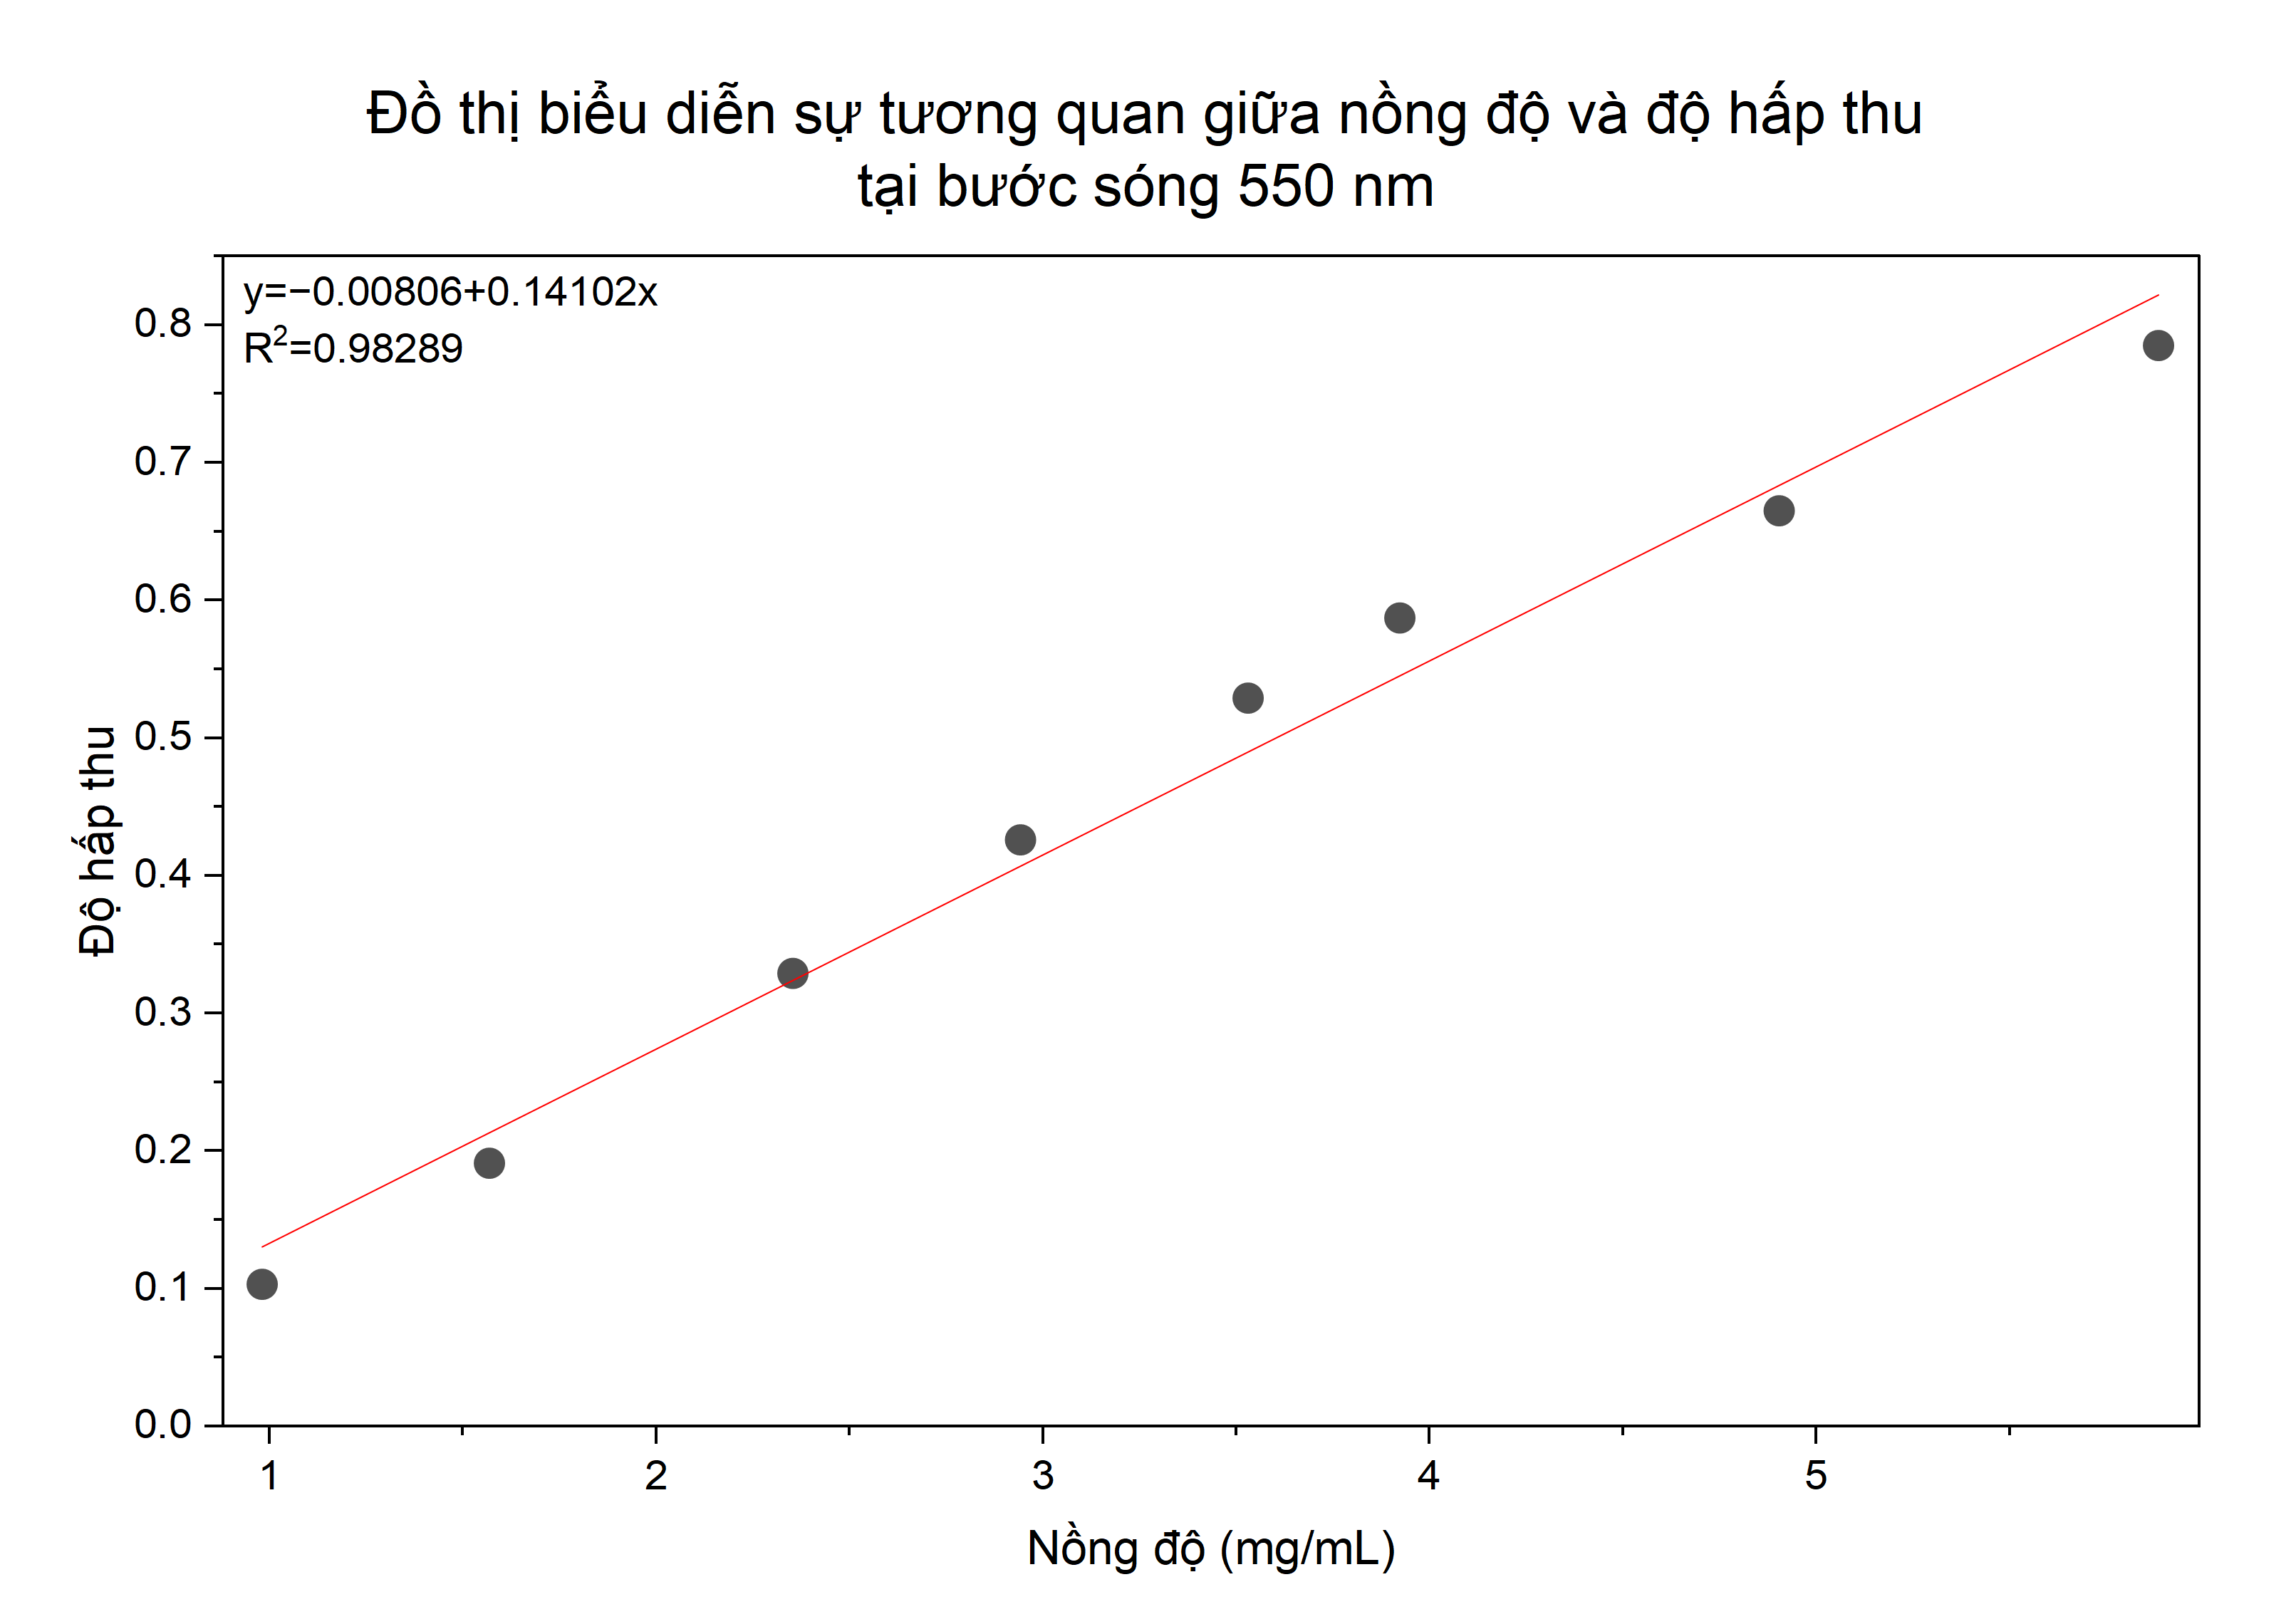
\includegraphics[scale=0.575]{image/danh gia xuc tac/duong chuan.png}
    \caption{\centering Đồ thị tương quan giữa nồng độ acetone và độ hấp thu ở bước sóng 550nm}
\end{figure}

\paragraph*{2.4.4. Hệ thống khí}
\leavevmode

Hệ thống được thiết lập nhằm mô phỏng điều kiện không khí thực tế với tỉ lệ thể tích $4N_2:1O_2$. Để đạt được nồng độ và độ ẩm mong muốn, các hợp chất hữu cơ dễ bay hơi (VOC) và hơi nước được bổ sung vào dòng khí bằng cách cho dòng $N_2$ lôi cuốn.

Quy trình vận hành bắt đầu bằng việc chia nguồn $N_2$ nguyên chất thành ba nhánh. Nhánh 1 dẫn dòng $N_2$ qua impinger chứa acetone được đặt trong bể điều nhiệt để lôi cuốn một lượng acetone xác định. Nhánh 2 dẫn dòng $N_2$ qua impinger chứa nước để tạo độ ẩm cho dòng hỗn hợp khí. Nhánh 3 dẫn dòng $N_2$ qua một lưu lượng kế để điều chỉnh lưu lượng dòng $N_2$ thay đổi nồng độ acetone trong dòng hỗn hợp khí. Sau đó, dòng $N_2$ này được trộn lẫn với dòng $O_2$ nguyên chất, tạo thành hỗn hợp khí đầu vào cho hệ thống như hình 2.5. 

\begin{figure}[H]
	\centering
    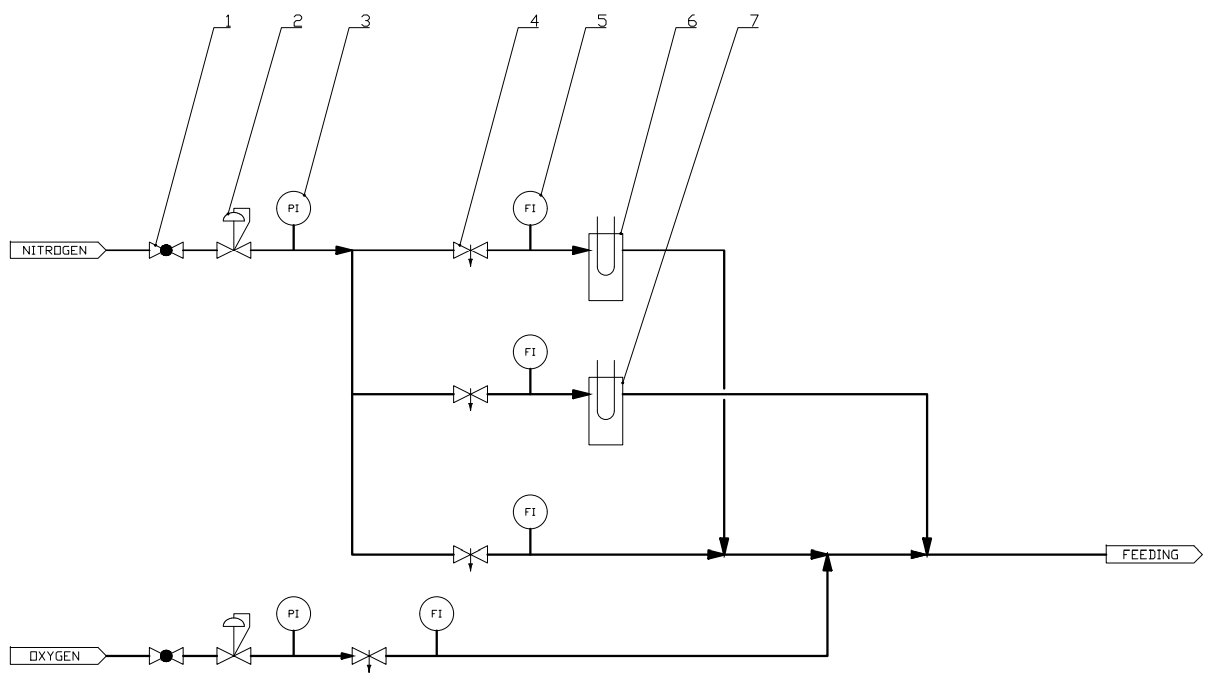
\includegraphics[scale=0.6]{image/chi tiet quy trinh/p&id feeding.png}
    \caption{\centering Quy trình hệ thống khí tạo dòng feeding chứa Acetone giả dòng không khí}
\end{figure}

\begin{enumerate}
    \item Van bi
    \item Van điều áp
    \item Áp kế
    \item Van kim
    \item Lưu lượng kế
    \item Impinger chứa acetone
    \item Impinger chứa nước.
\end{enumerate}

\paragraph*{2.4.5. Quy trình thực hiện}
\leavevmode

Vận hành hệ thống được miêu tả ở mục 2.4.4 với điều kiện thí nghiệm như sau

\begin{itemize}
    \item Nhiệt độ acetone trong bể điều nhiệt: $0^oC$
    \item Lưu lượng tổng: 625 mL/ph 
    \item Lưu lượng dòng khí $O_2$: 125 mL/ph 
    \item Lưu lượng dòng khí $N_2$ qua acetone: 25 mL/ph 
    \item Có ẩm. Lưu lượng dòng khí $N_2$ qua impinger chứa nước lần lượt là: 10 mL/ph và 20 mL/ph. %0 mL/ph,
    \item Lưu lượng dòng khí $N_2$ qua hỗn hợp khí: 465 mL/ph đối với dòng $N_2$ lôi cuốn hơi nước 10 mL/ph và 455 mL/ph đối với dòng $N_2$ lôi cuốn hơi nước 20 mL/ph. %475 mL/ph đối với dòng hỗn hợp không ẩm, 
\end{itemize}

Dẫn dòng khí đầu vào qua 1 bình erlen chứa 60ml dung dịch thuốc thử và 2 ống ly tâm chứa 30ml dung dịch thuốc thử ở mỗi ống trong khoảng thời gian xác định. Sau phản ứng đo độ hấp thu của dung dịch ở bình erlen đầu và ống ly tâm thứ 2 ở bước sóng 550 nm bằng máy quang phổ UV-Vis, riêng ống ly tâm thứ 3 đóng vai trò định tính (xem xét sự đổi màu cho thấy độ hấp thu của mẫu đo ở ống ly tâm này có giá trị gần bằng mẫu trắng). Dựa vào đường chuẩn đã xây dựng để xác định nồng độ acetone trong dòng khí dòng vào. Kết quả tại các trường hợp được trình bày tại mục 2.4.6. % không ẩm và có ẩm 

\paragraph*{2.4.6. Kết quả tính toán}
\leavevmode

Kết quả đo độ hấp thu được thể hiện ở bảng 2.7:

\begin{table}[H]
    \centering
    \begin{tabular}{@{}|
                >{\centering\arraybackslash}m{1.75cm}|    
                >{\centering\arraybackslash}m{3.5cm}|
                >{\centering\arraybackslash}m{2.2cm}|
                >{\centering\arraybackslash}m{2.3cm}|
                >{\centering\arraybackslash}m{1.5cm}|
                >{\centering\arraybackslash}m{2.1cm}|@{}} \hline
        \textbf{Trường hợp} & \textbf{Dòng $N_2$ lôi cuốn hơi nước (mL/ph)} & \textbf{Thời gian (ph)} & \textbf{Thể tích mỗi bình (mL)} & \textbf{Độ hấp thu} & \textbf{Nồng độ acetone (mg/mL)} \\ \hline
        % \multirow{2}{*}{\makecell{Không\\ẩm}} &
        % \multirow{2}{*}{0} &
        % \multirow{2}{*}{10} & \centering 60 & 0,683 & 4,9050\\ \cline{4-6}
        %  & & & \centering 30 & 0,264 & 1,9333\\ \hline
        \multirow{4}{*}{\makecell{Có\\ẩm}} &
        \multirow{2}{*}{10} &
        \multirow{2}{*}{5} & \centering 60 & 0,587 & 4,2241\\ \cline{4-6}
         & & & \centering 30 & 0,204 & 1,5078\\ \cline{2-6}
         & \multirow{2}{*}{20} &
        \multirow{2}{*}{3,5} & \centering 60 & 0,464 & 3,3518\\ \cline{4-6}
         & & & \centering 30 & 0,166 & 1,2383\\ \hline
    \end{tabular}
    \caption{\centering Kết quả đo nồng độ dòng khí đầu vào trước khi đưa qua bình phản ứng tại các điều kiện không ẩm và có ẩm tại T = $0^oC$}
\end{table}

% a) Không ẩm

Thực hiện tính toán nồng độ acetone trong dòng hỗn hợp khí đầu vào tại điều kiện có ẩm với điều kiện lưu lượng dòng $N_2$ lôi cuốn hơi nước là 10ml trong dòng khí, ta được: 

Lượng acetone bị giữ lại trong pha lỏng ở bình 1 ($V_1 = 60$ mL) trong 10 phút:

\begin{center}
    $n_1 = C_1 \times V_1 = 4,2241 \times 60 = 253,446 \ (mg)$
\end{center}

Lượng acetone bị giữ lại trong pha lỏng ở bình 2 ($V_2 = 30$ mL) trong 10 phút:

\begin{center}
    $n_2 = C_2 \times V_2 = 1,5078 \times 30 = 45,234 \ (mg)$
\end{center}

Tổng lượng acetone bị giữ lại trong pha lỏng trong 1 phút:

\begin{center}
    $n = \dfrac{n_1 + n_2}{10} = \dfrac{253,446 + 45,234}{5} = 59,736 \ (mg)$
\end{center}

Thể tích lượng hơi acetone bị lôi cuốn trong 1 phút ở điều kiện tiêu chuẩn:

\begin{center}
    $V = \dfrac{nRT}{MP} = \dfrac{59,736 \times 10^{-3} \times 0,082 \times 298}{58 \times 1} = 0,0252 \ (L)$
\end{center}

Nồng độ acetone trong hỗn hợp khí:

\begin{center}
    $C = \dfrac{V}{\sum V} = \dfrac{0,0252 \times 10^3}{625} \times 10^6 = 40268 \ (mL/m^3) = 40268 \ ppm$
\end{center}%

% b) Có ẩm

Tương tự như khi tính toán với trường hợp có ẩm với lưu lượng dòng $N_2$ lôi cuốn hơi nước là 20ml thu được kết quả về nồng độ acetone là 45888 ppm.

Sau khi tiến hành tại điều kiện nhiệt độ T = $0^oC$, nhận thấy nồng độ acetone trong dòng hỗn hợp khí đầu vào khá cao nên tiến hành giảm nhiệt độ xuống T = $-10^oC$. Đo và khảo sát kết quả như tại nhiệt độ T = $0^oC$, thu được các giá trị theo bảng sau:

\begin{table}[H]
    \centering
    \begin{tabular}{@{}|
                >{\centering\arraybackslash}m{1.75cm}|    
                >{\centering\arraybackslash}m{2.0cm}|
                >{\centering\arraybackslash}m{1.3cm}|
                >{\centering\arraybackslash}m{2.1cm}|
                >{\centering\arraybackslash}m{1.5cm}|
                >{\centering\arraybackslash}m{2.1cm}|
                >{\centering\arraybackslash}m{2.1cm}|@{}} \hline
        \textbf{Trường hợp} & \textbf{Dòng $N_2$ lôi cuốn hơi nước (mL/ph)} & \textbf{Thời gian (ph)} & \textbf{Thể tích mỗi bình (mL)} & \textbf{Độ hấp thu} & \textbf{Nồng độ acetone pha lỏng (mg/mL)} & \textbf{Nồng độ acetone trong dòng hỗn hợp khí (ppm)} \\ \hline
        % \multirow{2}{*}{\makecell{Không\\ẩm}} &
        % \multirow{2}{*}{0} &
        % \multirow{2}{*}{10} & \centering 60 & 0,297 & 2,1674 & \multirow{2}{*}{12346,0066}\\ \cline{4-6}
        %  & & & \centering 30 & 0,241 & 1,7702 & \\ \hline
        \multirow{4}{*}{\makecell{Có\\ẩm}} &
        \multirow{2}{*}{10} &
        \multirow{2}{*}{5} & \centering 60 & 0,317 & 2,3092 & \multirow{2}{*}{23028,2856}\\ \cline{4-6}
         & & & \centering 30 & 0,143 & 1,0752 &\\ \cline{2-7}
         & \multirow{2}{*}{20} &
        \multirow{2}{*}{3,5} & \centering 60 & 0,260 & 1,9050 & \multirow{2}{*}{26586,8597}\\ \cline{4-6}
         & & & \centering 30 & 0,103 & 0,7915 &\\ \hline
    \end{tabular}
    \caption{\centering Kết quả đo nồng độ dòng khí đầu vào trước khi đưa qua bình phản ứng tại các điều kiện có ẩm tại T = $-10^oC$} % không ẩm và
\end{table}

Nhận thấy kết quả đo tại T = $-10^oC$ cho ra nồng độ acetone trong dòng hỗn hợp khí đầu vào đã giảm đi khá nhiều so với điều kiện trước đó. Tiến hành thu thập kết quả và sử dụng để nghiên cứu độ chuyển hoá cho quá trình oxi hoá sâu acetone.


\subsection*{4. Kết quả và thảo luận}
\phantomsection \addcontentsline{toc}{subsection}{\bfseries \numberline{}4. Kết quả và thảo luận}
\setcounter{section}{4}
\setcounter{figure}{0}
\setcounter{table}{0}
\subsubsection*{4.1. Kết quả}
\phantomsection \addcontentsline{toc}{subsubsection}{\numberline{}4.1. Kết quả}

\paragraph*{4.1.1. Scanning electron microscopy (SEM)}
\leavevmode

Hình thái của Cu-doped cryptomelane được thể hiện trên hình 4.1. Kết quả cho thấy Cu-doped cryptomelane có cấu trúc dạng thanh nano (nanorods) phân bố đồng đều với đường kính các thanh dao động trong khoảng từ 14 - 40 nm. Khi quan sát ở độ phóng đại $10 \ \mu m$ (hình 4.1b), ta có thể nhận thấy các thanh nano này có xu hướng kết tụ thành các mảng lớn.

Sự kết tụ quan sát được trong ảnh SEM (hình 4.1b) có thể được giải thích thông qua cơ chế năng lượng bề mặt. Các nanorods có kích thước nhỏ nên năng lượng bề mặt của chúng rất lớn. Để bền vững hơn theo nguyên tắc nhiệt động lực học, các thanh nano đơn lẻ có xu hướng giảm thiểu năng lượng tự do (free enthalpy - G) này bằng cách tự liên kết và kết tụ lại với nhau tạo thành các bó hoặc mảng lớn \cite{13}. Ngoài ra, theo Awaluddin và các cộng sự \cite{15}, không có sự thay đổi đáng kể về hình thái giữa mẫu tinh khiết và các mẫu pha tạp $Cu^{2+}$ với các nồng độ khác nhau, tất cả đều tồn tại dưới dạng các khối kết tụ. Sự tương đồng này cho thấy việc thay đổi nồng độ ion $Cu^{2+}$ không làm thay đổi cơ chế phát triển hình thái của vật liệu.

So sánh với bề mặt của màng Cu-doped cryptomelane được thể hiện qua hình 4.2. Ở độ phóng đại 500 nm (hình 4.2a), vật liệu vẫn duy trì cấu trúc dạng thanh nano đặc trưng tương tự như mẫu bột. Tuy nhiên, các thanh nano trên mẫu màng giờ đây có sự liên kết chặt chẽ, sắp xếp đan xen và chồng chất lên nhau khác hẳn với dạng rời rạc trong dạng bột. Quan sát tổng thể ở độ phóng đại $10 \ \mu m$ (hình 4.2b), các thanh nano này phân bố đồng đều và liên kết tạo thành một cấu trúc mạng lưới xốp liên tục thống nhất thay vì các khối cục bộ. Việc tạo ra cấu trúc xốp này có lợi cho diện tích xúc tác vì nó vừa đảm bảo tính liên kết của màng, vừa duy trì được các khoảng trống kích thước nano giữa các thanh.

\begin{figure}[H]
	\centering
    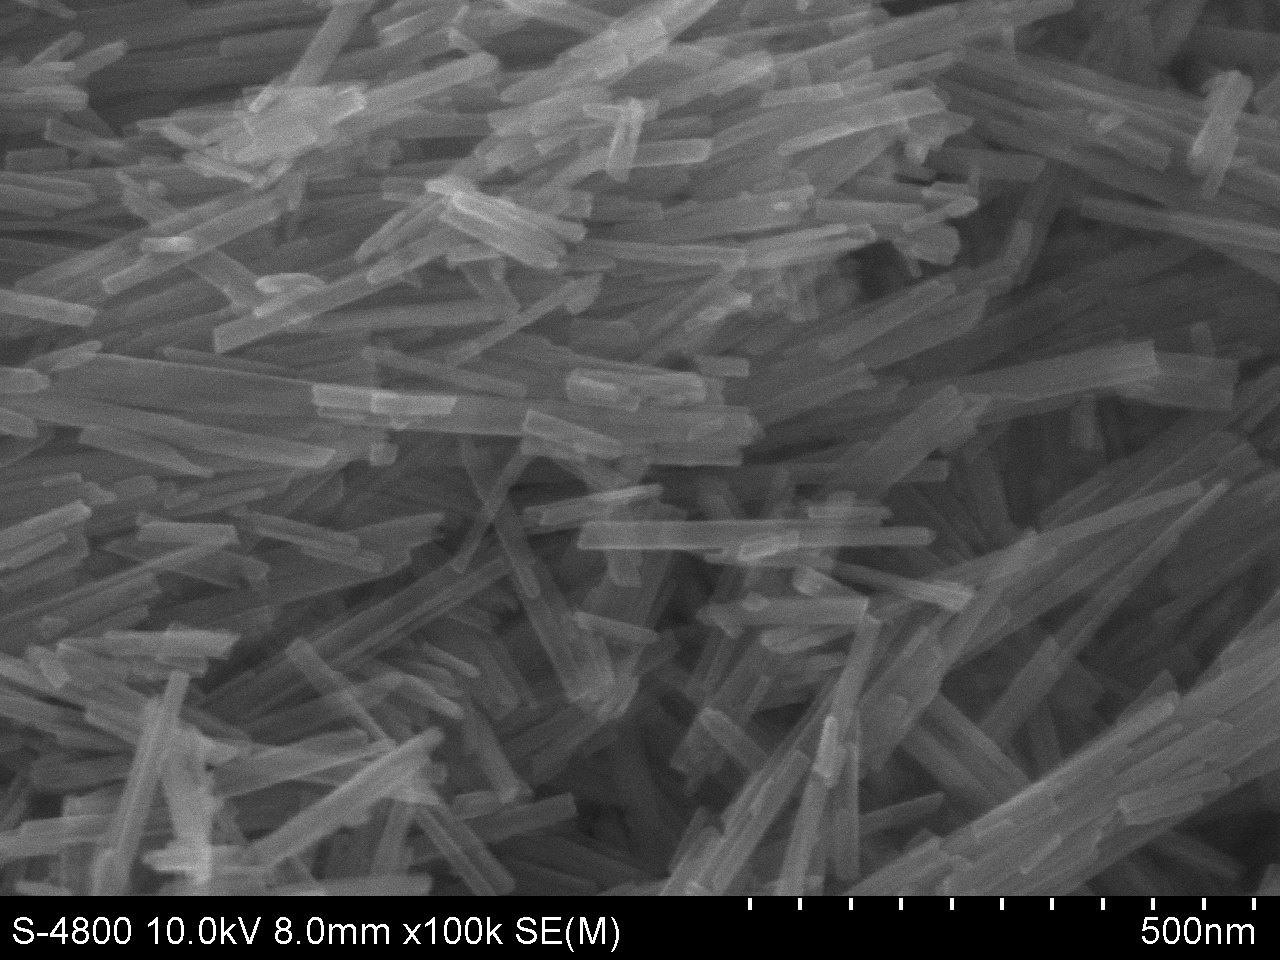
\includegraphics[scale=0.125]{image/ket qua/1_m08.png}
    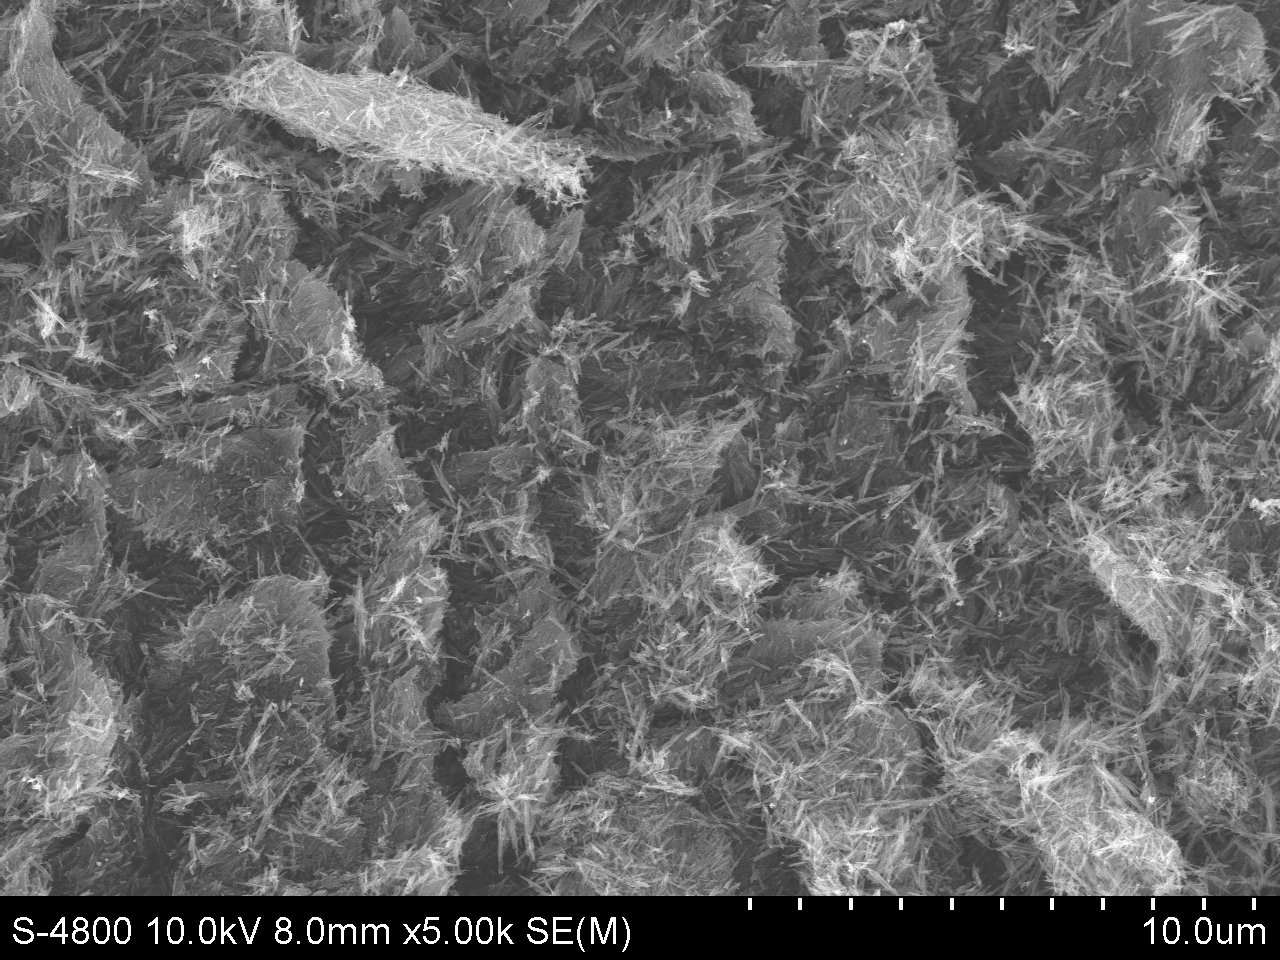
\includegraphics[scale=0.125]{image/ket qua/1_m05.png}
    \caption{\centering Hình ảnh SEM của mẫu bột Cu-doped cryptomelane với độ phóng đại: $a) \ 500 \ nm, \ b) \ 10 \ \mu m$}
\end{figure}

\begin{figure}[H]
	\centering
    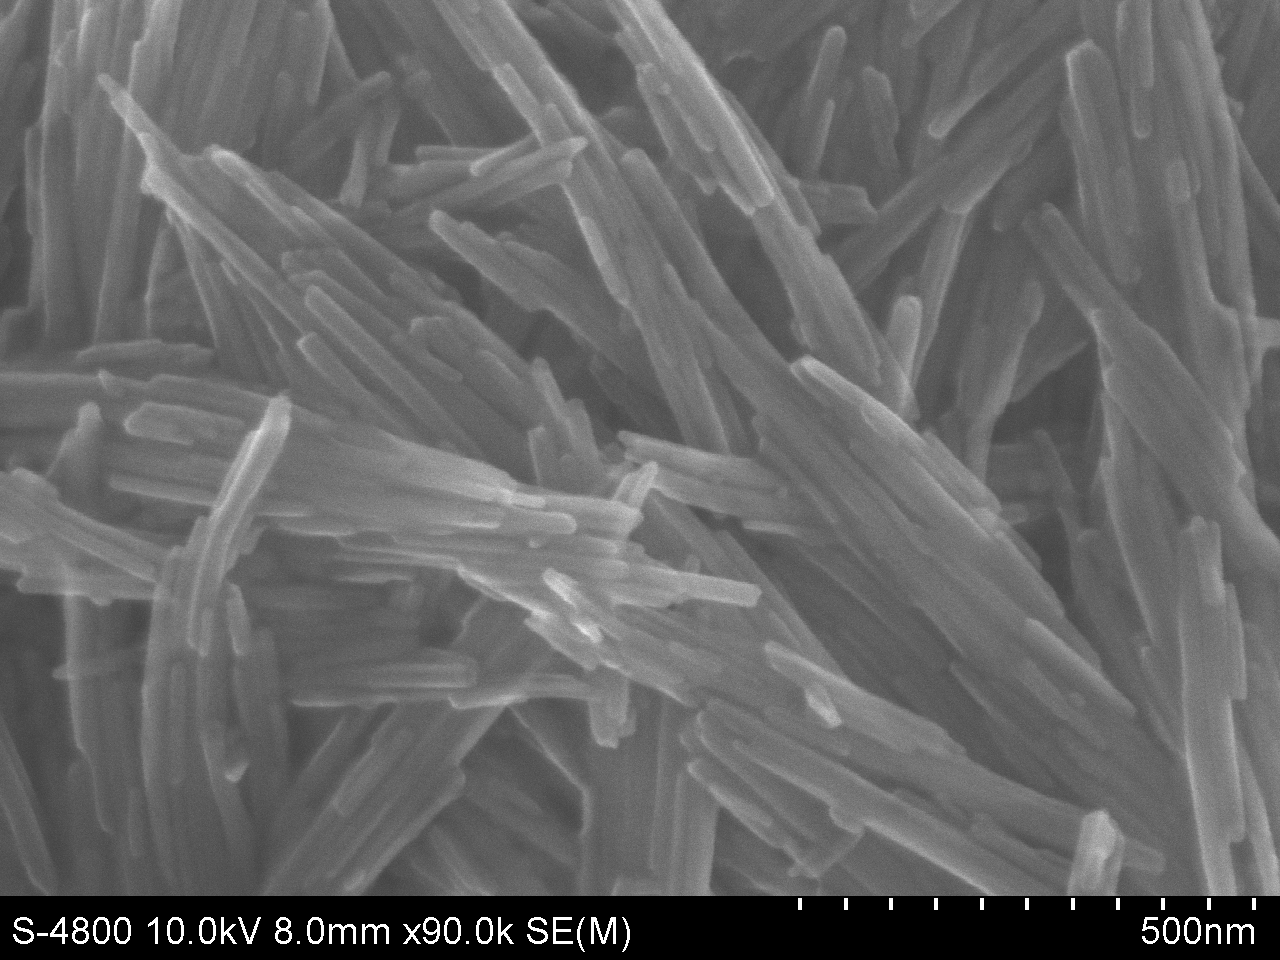
\includegraphics[scale=0.125]{image/ket qua/1_m05_2.png}
    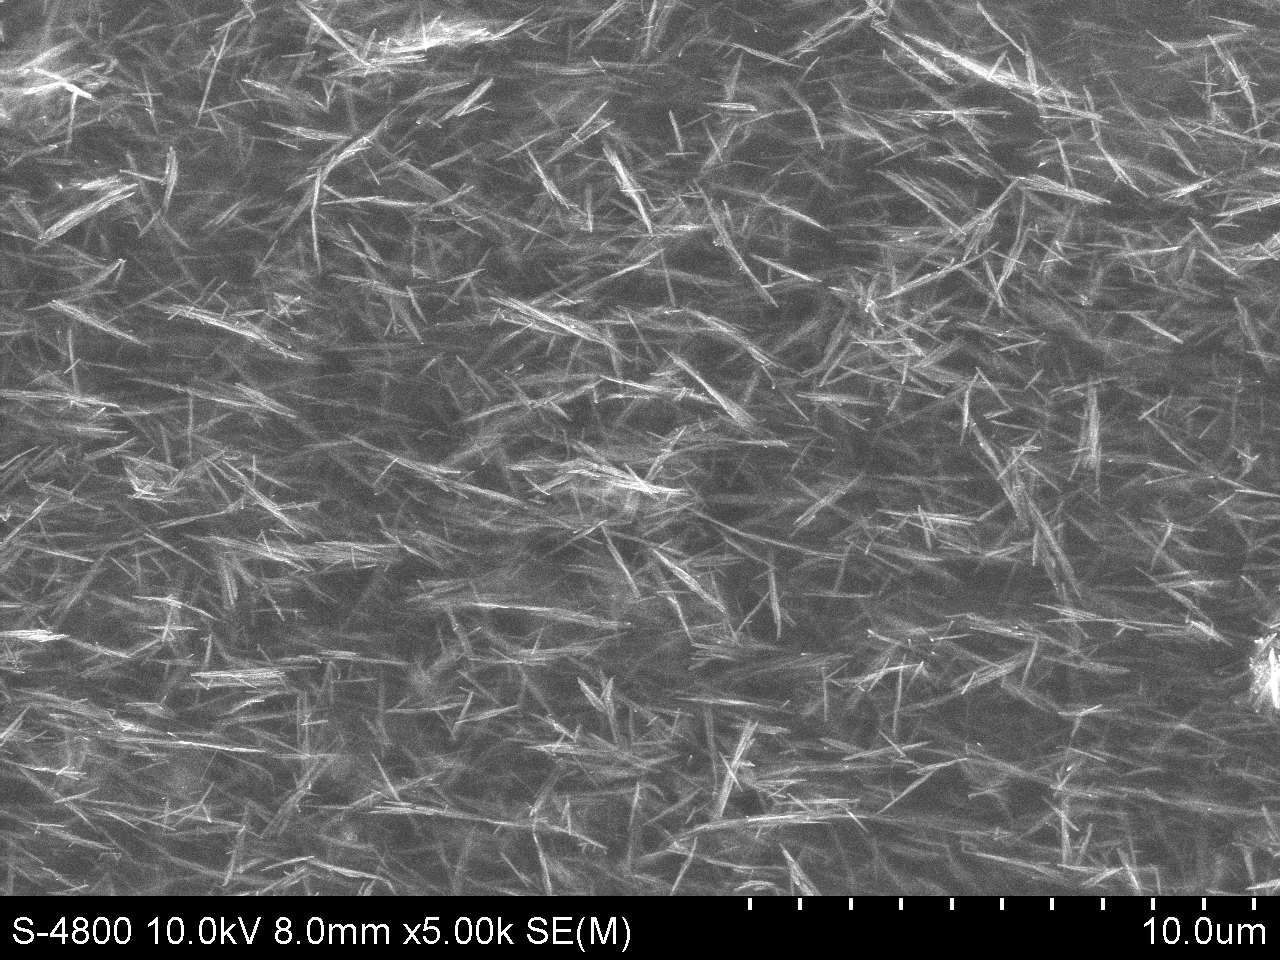
\includegraphics[scale=0.125]{image/ket qua/1_m04.png}
    \caption{\centering Hình ảnh SEM của mẫu màng Cu-doped cryptomelane với độ phóng đại: $a) \ 500 \ nm, \ b) \ 10 \ \mu m$}
\end{figure}

Tiến hành việc thu thập kích thước hạt tinh thể trên mẫu bột trên các thang đo 200nm, 500nm, 1um với cỡ mẫu khảo sát là N = 162. Sau đó kiểm định tính chuẩn với giả thuyết đưa ra là dữ liệu về phân bố kích thước hạt tuân theo phân phối chuẩn, thu được kết quả như sau:

\begin{figure}[H]
	\centering
    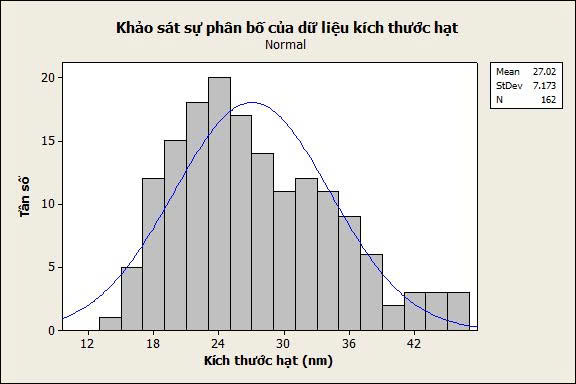
\includegraphics[scale=0.6]{image/ket qua/size distribution/anh xac dinh tinh chuan phan bo kich thuoc hat.jpg}

    \vspace{6pt}
    
    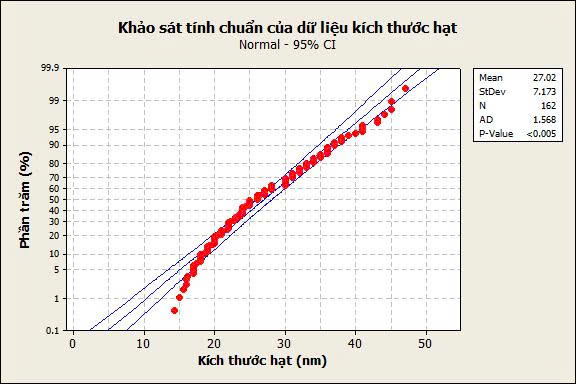
\includegraphics[scale=0.6]{image/ket qua/size distribution/anh xac dinh tinh chuan kich thuoc hat.jpg}
    \caption{\centering Khảo sát tính chuẩn của dữ liệu kích thước hạt}
\end{figure}

Với đồ thị phân bố kích thước hạt như trên, từ khoảng 13-19 nm có 18 hạt mang khoảng kích thước này. Với miền giá trị kích thước lớn (37-47 nm) có 17 giá trị nằm trong khoảng kích thước này. Khi xét cỡ mẫu N = 162 hạt, rõ ràng các vùng kích thước ngoại lai này chiếm tỉ lệ số hạt khá thấp (11.1\% và 10.5\%) cho thấy phần lớn số hạt có kích thước trong khoảng từ 19 tới 36 nm (127/162 hạt). Đây là miền tập trung của các hạt, cho thấy hạt phân bố kích thước khá đồng đều. Bên cạnh đó, giá trị trung bình là Mean = 27.02 với độ lệch chuẩn là 7.173 càng chứng tỏ miền giá trị kích thước nằm trong khoảng đang xét.

Sau khi tiến hành xác định sự phân bố kích thước hạt và kiểm định tính chuẩn của tập dữ liệu này, với giả thuyết $H_o$ là dữ liệu tuân theo phân phối chuẩn, giá trị $p_{value}$ thu được với cỡ mẫu N = 162 là rất nhỏ (< 0.005), chứng tỏ giả thuyết ban đầu là sai và tập dữ liệu không tuân theo phân phối chuẩn.

Tuy nhiên, khi tham khảo các nghiên cứu liên quan, dữ liệu kích thước hạt phân tích từ ảnh SEM thường tuân theo quy luật phân phối Lognormal. Đây là dạng phân phối đặc trưng với đỉnh dữ liệu lệch về phía trái và phần đuôi bên phải kéo dài. Quan sát biểu đồ tần suất (Histogram) tại hình 4.4, dữ liệu thực nghiệm cho thấy sự tương thích cao với mô hình này. Do đó, quá trình phân tích tiếp theo được thực hiện dựa trên giả định phân phối Lognormal và thu được kết quả như sau:

\begin{figure}[H]
	\centering
    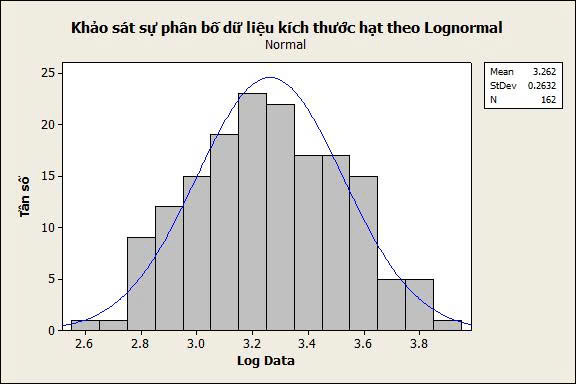
\includegraphics[scale=0.6]{image/ket qua/size distribution/anh xac dinh su phan bo kich thuoc hat theo lognormal.jpg}

    \vspace{6pt}

    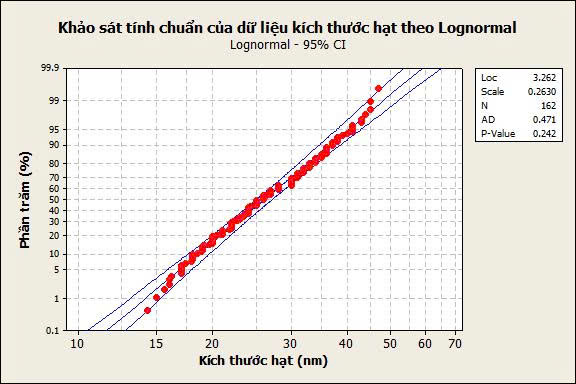
\includegraphics[scale=0.6]{image/ket qua/size distribution/anh xac dinh tinh chuan kich thuoc hat theo lognormal.jpg}
    \caption{\centering Khảo sát tính chuẩn của dữ liệu kích thước hạt theo phân phối Lognormal}
\end{figure}

Qua sự khảo sát theo hai dạng phân phối như trên, có thể xác định dữ liệu kích thước các hạt tinh thể Cu-OMS-2 tuân theo phân phối Lognormal với giá trị $p_{value}$ cho giả thuyết H$_o$ (dữ liệu tuân theo phân phối Lognormal) là khá cao ($p_{value}$ = 0.242). Việc xác định kích thước các hạt tuân theo phân phối Lognormal phần nào giải thích được quá trình nghiền hạt là đúng, vì trong tự nhiên các quá trình nghiền bi hạt từ kích thước lớn hơn sang các hạt có kích thước nhỏ hơn làm cho dữ liệu về kích thước các hạt thường tuân theo phân phối Lognormal \cite{23}. Ngoài ra dạng phân phối Lognormal cho thấy phần lớn các hạt có kích thước nhỏ, do đó diện tích bề mặt hấp phụ lớn hơn làm tăng hiệu suất phản ứng \cite{24}.

\paragraph*{4.1.2. X-ray diffraction (XRD)}
\leavevmode

Cấu trúc pha và độ tinh khiết của các mẫu bột Cu-OMS-2 sau tổng hợp được thể hiện thông qua các giản đồ nhiễu xạ tia X (XRD) trong hình 4.5. So sánh với dữ liệu chuẩn crytomelane JCPDS 029 - 1020, các mẫu bột Cu-OMS-2 với nồng độ $Cu^{2+}$ pha tạp khác nhau đều cho ra các đỉnh nhiễu xạ đặc trưng khá tương đồng tại các góc $2 \theta$ lần lượt là $12.79^{\circ}, 18.17^{\circ}, 28.79^{\circ}, 37.58^{\circ}, 41.84^{\circ}, 49.82^{\circ}$ và $60.12^{\circ}$, tương ứng với các mặt mạng (110), (200), (310), (211), (301), (411) và (521).

\begin{figure}[H]
	\centering
    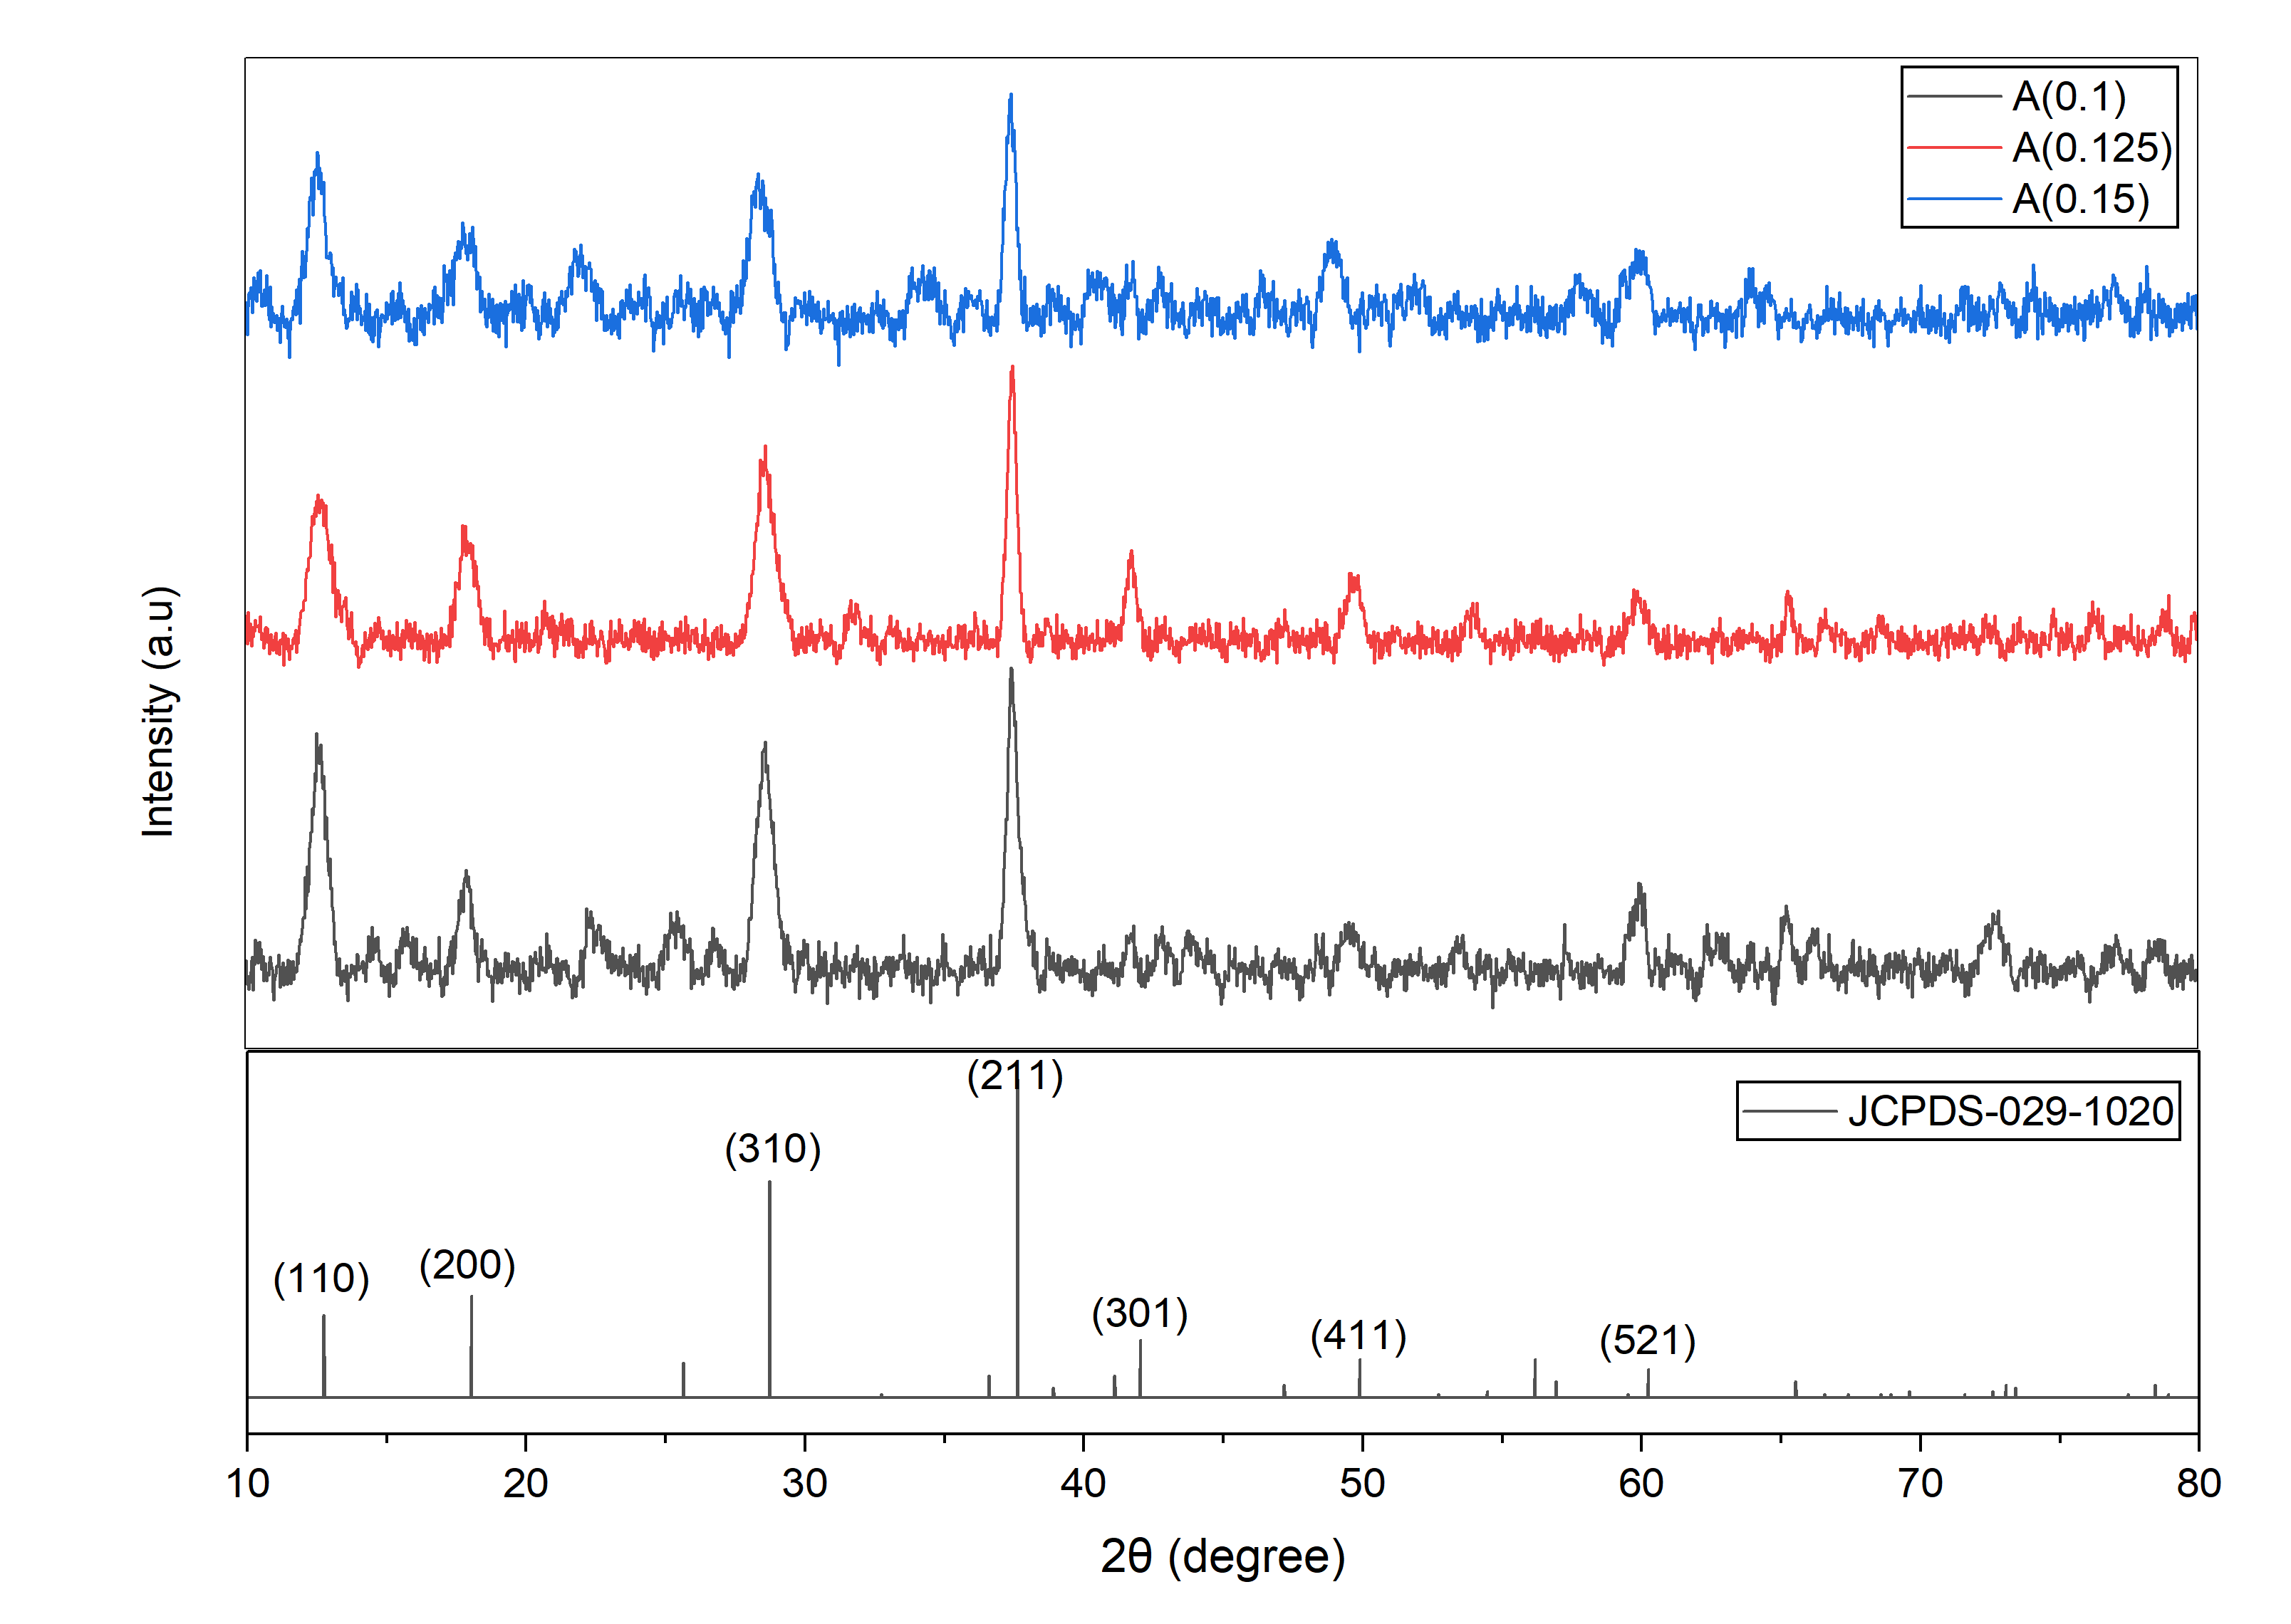
\includegraphics[scale=0.5]{image/danh gia xuc tac/XRD.png}
    \caption{\centering Khảo sát phổ X-ray diffraction của Cu-OMS2 tại các nồng độ khác nhau}
\end{figure}

Dựa theo giản đồ nhiễu xạ, không phát hiện thấy các đỉnh lạ nào khác xuất hiện do việc kết hợp $Cu^{2+}$ ở các nồng độ khác nhau, điều này cho thấy các ion $Cu^{2+}$ kết hợp tốt vào bên trong mạng lưới tinh thể của cryptomelane thay vì làm thay đổi cấu trúc vi mô bên ngoài, luận điểm này càng được củng cố thêm bằng việc ảnh SEM không có sự thay đổi đáng kể về hình thái khi pha tạp lượng $Cu^{2+}$ khác nhau (như đã phân tích ở phần 4.1.1). Ngoài ra, các kết quả tương tự cũng được báo cáo bởi Gao \cite{21} và Ma \cite{22} sau khi thêm các kim loại chuyển tiếp khác nhau (Fe, Co, Ni và Cu) vào cryptomelane nguyên chất. Trong hình 4.5 cũng chỉ ra rằng cường độ tương đối các đỉnh nhiễu xạ của cryptomelane pha tạp Cu dần trở nên yếu hơn theo thứ tự cường độ peak A(0,1) > A(0,125) > A(0,15) (tức là lượng Cu càng nhiều thì đỉnh càng thấp, càng bị bè ra). Điều này cho thấy rằng các biến dạng của cryptomelane tinh khiết đã được tạo ra khi chất pha tạp kết hợp vào mạng lưới, hiện tượng này cũng được quan sát bởi Awaluddin \cite{15} và Gao \cite{21}.

\paragraph*{4.1.3. Phân tích nguyên tố}
\leavevmode

Quy trình xử lí mẫu trước khi đem đo bao gồm các quy trình chính sau. Đầu tiên, mẫu được cân với khối lượng 0,1000g sau đó được hoà tan cùng 5ml dung dịch axit nitric đậm đặc và 2ml $H_2O_2$ 30\%. Sau đó pha loãng dung dịch thu được tới 50ml thể tích. Tiến hành lưu mẫu và đem đi đo tại Trung tâm Phân tích Tự nhiên - Trường Đại học Khoa học Tự nhiên Thành phố Hồ Chí Minh do PGS.TS. Nguyễn Văn Đông phụ trách.

Kết quả phân tích nguyên tố Cu và Mn của OMS-2 và Cu-OMS-2 được trình bày trong bảng 4.1. Ở các nồng độ chất pha tạp cao hơn, có sự tăng nồng độ Cu phù hợp với sự tăng nồng độ Cu tiền chất. Đối với Mn, nồng độ Mn giảm đều, cho thấy rằng các ion Cu đang thay thế Mn trong khung mạng của OMS-2.

\begin{table}[H]
    \centering
    \begin{tabular}{@{}|c|p{1.75cm}|p{1.75cm}|p{1.75cm}|p{1.75cm}|c|@{}} \hline
        \textbf{Mẫu} & \multicolumn{2}{p{3.5cm}|}{\centering \textbf{Cu}} & \multicolumn{2}{p{3.5cm}|}{\centering \textbf{Mn}} & \textbf{$n_{Cu}/n_{Mn}$} \\ \cline{2-5}
         & \centering \textbf{ppm} & \centering \textbf{mg} & \centering \textbf{ppm} & \centering \textbf{mg} & \\ \hline
        K-OMS-2 & \centering 0 & \centering 0 & \centering 1093,6 & \centering 54,68 & 0 \\ \hline
        Cu-OMS-2 (0,1M) & \centering 41,49 & \centering 2,075 & \centering 1054,0 & \centering 52,7 & 0,033 \\ \hline
        Cu-OMS-2 (0,125M) & \centering 43,12 & \centering 2,156 & \centering 1039,3 & \centering 51,965 & 0,037 \\ \hline
        Cu-OMS-2 (0,15M) & \centering 50,27 & \centering 2,514 & \centering 1021,1 & \centering 51,055 & 0,042 \\ \hline
    \end{tabular}
    \caption{\centering Kết quả phân tích nguyên tố Cu và Mn của OMS-2 và Cu-OMS-2}
\end{table}

Điều này tương đối phù hợp với nghiên cứu \cite{15} của Awaluddin. Theo Awaluddin, sự thay thế cho một số ion mangan trong khung mạng của oxit mangan sẽ chủ yếu diễn ra khi nồng độ ion $Cu^{2+}$ lúc tổng hợp còn thấp ($n_{Cu}/n_{Mn}<0,0301$), chứ không thay thế cho các ion $K^{+}$ trong các vị trí đường hầm. Khi có nhiều ion $Cu^{2+}$ ($n_{Cu}/n_{Mn}>0,0301$) được thêm vào trong quá trình tổng hợp, các ion $Cu^{2+}$ thay thế cho một số ion $K^{+}$ trong các vị trí đường hầm. Có thể việc thay thế $K^+$ diễn ra đồng thời với việc thay thế ion Mn nên lượng ion $Cu^{2+}$ tăng mạnh hơn.

Bên cạnh đó, với việc thành phần phần trăm khối lượng của Cu và Mn lần lượt là 2,075 -- 2,515 \% và 51,055 -- 52,7 \% phù hợp cấu trúc lý thuyết của Cryptomelane đồng thời khẳng định quá trình pha tạp đã diễn ra thành công.

\paragraph*{4.1.4. Xác định trạng thái oxy hoá trung bình của Mangan}
\leavevmode

Kết quả xác định trạng thái oxy hoá trung bình của Mangan trong OMS-2 và Cu-OMS-2 được thể hiện trong bảng 4.2. Các giá trị số oxy hóa trung bình (Average Oxidation State - AOS) dao động từ 3,65 đến 3,75 cho thấy sự phù hợp đối với các loại vật liệu Cryptomelane.

\begin{table}[H]
    \centering
    \begin{tabular}{@{}|c|c|p{1.25cm}|p{2.55cm}|p{2.7cm}|c|@{}} \hline
        \multirow{2}{*}{\textbf{Mẫu}} & \centering \textbf{\%Mn} & \centering \textbf{$m_{\text{mẫu}}$} & \centering \textbf{$V_{Na_2S_2O_3 \text{(mẫu)}}$} & \centering \textbf{$V_{Na_2S_2O_3 \text{(trắng)}}$} & \multirow{2}{*}{\textbf{AOS}} \\
         & \centering \textbf{(\%w/w)} & \centering \textbf{(g)} & \centering \textbf{(mL)} & \centering \textbf{(mL)} & \\ \hline
        K-OMS-2 & \centering 54,68 & \centering 0,0502 & \centering 8,350 & \centering 0,1 & 3,65 \\ \hline
        Cu-OMS-2 (0,1M) & \centering 52,7 & \centering 0,0508 & \centering 8,600 & \centering 0,1 & 3,75 \\ \hline
        Cu-OMS-2 (0,125M) & \centering 51,965 & \centering 0,0498 & \centering 8,325 & \centering 0,1 & 3,75 \\ \hline
        Cu-OMS-2 (0,15M) & \centering 51,055 & \centering 0,0506 & \centering 8,350 & \centering 0,1 & 3,76 \\ \hline
    \end{tabular}
    \caption{\centering Kết quả xác định AOS của Mangan của OMS-2 và Cu-OMS-2}
\end{table}

Khi so sánh giữa các mẫu, có thể thấy rõ xu hướng gia tăng chỉ số AOS sau khi pha tạp ion kim loại chuyển tiếp ($Cu^{2+}$). Cụ thể, mẫu K-OMS-2 có AOS đạt 3,65, trong khi các mẫu pha tạp đồng Cu-OMS-2 (0,1M; 0,125M và 0,15M) đều ghi nhận mức AOS cao hơn, đạt 3,75. Kết quả này hoàn toàn phù hợp với nghiên cứu \cite{25} cho thấy sự hiện diện của các chất pha tạp làm tăng dần AOS theo thứ tự từ mẫu K-OMS-2 < Co-OMS-2 < Cu-OMS-2.

Sự gia tăng của AOS được giải thích là kết quả của việc sụt giảm tỷ lệ Mn(III)/Mn(IV) trong cấu trúc vật liệu. Các ion $Cu^{2+}$ khi được đưa vào quá trình tổng hợp có khả năng thay thế một phần các ion Mn có số oxy hóa thấp ($<4+$) trong liên kết Mn-O của khung mạng. Ngoài ra, một lượng nhất định ion $Cu^{2+}$ cũng có thể thay thế các ion $K^+$ tại vị trí đường hầm để bù trừ điện tích âm cho lớp. Quá trình thay thế này không chỉ làm tăng trạng thái oxy hóa trung bình của Mangan tiến sát về mức lý tưởng (+4) mà còn có thể tạo ra thêm các lỗ hổng oxy, đóng vai trò then chốt trong việc tăng cường hoạt tính xúc tác oxy hóa của vật liệu.

\subsubsection*{4.2. Thảo luận}
\phantomsection \addcontentsline{toc}{subsubsection}{\numberline{}4.2. Thảo luận}
\cleardoublepage

\section*{KẾT LUẬN}
\phantomsection \addcontentsline{toc}{section}{\numberline{}KẾT LUẬN}

Nghiên cứu này đã thành công trong việc pha tạp đồng (Cu) vào vật liệu cryptomelane (OMS-2) để làm xúc tác cho quá trình oxi hoá sâu acetone. Ngoài ra còn đưa xúc tác Cu-OMS2 làm biến tính màng chitosan cùng với cellulose và đánh giá đặc trưng cấu trúc, hình thái bề mặt vật liệu.

1. Cấu trúc tinh thể

\hspace{0.5cm}- Phân tích giản đồ nhiễu xạ tia X (XRD) cho thấy vật liệu OMS-2 và Cu-OMS-2 đều có các đỉnh nhiễu xạ điển hình của cryptomelane, ngoài ra còn có các đỉnh nhiễu xạ khác do pha tạp oxit của đồng.

\hspace{0.5cm}- Các đỉnh nhiễu xạ của Cu-OMS-2 với các nồng độ khác nhau nhìn chung không dịch chuyển quá nhiều so với OMS-2, chứng tỏ việc pha tạp đồng không làm thay đổi cấu trúc tinh thể cơ bản của cryptomelane.

2. Hình thái bề mặt

\hspace{0.5cm}- Mẫu OMS-2, các mẫu Cu-OMS-2 khi ở dạng bột và khi đính lên màng nhìn chung đều có hình dạng bó sợi.

\hspace{0.5cm}- Các sợi có xu hướng kết tụ nhiều hơn đối với trường hợp OMS-2 và phân tán tốt hơn khi pha tạp với đồng (Cu).

Tóm lại, nghiên cứu đã ban đầu xác định và đánh giá được các đặc trưng cấu trúc, hình thái bề mặt của vật liệu Cu-OMS-2 và màng chitosan biến tính bởi cellulose và Cu-OMS-2. Sau khi hoàn thành phần đồ án chuyên ngành, nhóm em sẽ tiến hành khảo sát hoạt tính của xúc tác trong việc oxi hoá sâu acetone dưới các điều kiện về dòng khí cũng như môi trường (nhiệt độ, áp suất).

\cleardoublepage

\phantomsection \addcontentsline{toc}{section}{\numberline{}TÀI LIỆU THAM KHẢO}

\begin{thebibliography}{99}

\bibitem{1}
Canadian Centre for Occupational Health and Safety. (2023).  
\textit{Acetone}.

\url{https://www.ccohs.ca/oshanswers/chemicals/chem_profiles/acetone.html}

\bibitem{2}
Agency for Toxic Substances and Disease Registry. (1994).  
\textit{PUBLIC HEALTH STATEMENT
ACETONE}.

\url{https://www.atsdr.cdc.gov/ToxProfiles/tp21-c1-b.pdf}

\bibitem{3}
Darcel, C. (2023).  
\textit{An introduction to acetone: Everything you need to know}.

\url{https://www.maratek.com/blog/an-introduction-to-acetone-everything-you-need-to-know}

\bibitem{4}
PharmaCompass. (n.d.).  
\textit{Dimethylformaldehyde}. Retrieved November 23, 2025.

\url{https://www.pharmacompass.com/chemistry-chemical-name/dimethylformaldehyde}

\bibitem{5}
National Center for Biotechnology Information (2025). PubChem Compound Summary for CID 180, Acetone. Retrieved November 23, 2025.

\url{https://pubchem.ncbi.nlm.nih.gov/compound/Acetone}

\bibitem{6}
Kharlamova, T. S., Verkhov, V. A., Kulchakovskaya, E. V., Svetlichnyi, V. A., Aires, F. J. C. S., Bargiela, P., \& Vodyankina, O. V. (2022). \textit{Effect of metal-doping (Me = Fe, Ce, Sn) on phase composition, structural peculiarities, and CO oxidation catalytic activity of cryptomelane-type $MnO_{2}$}. Journal of Alloys and Compounds, 917, 165504.

\url{https://hal.science/hal-03764733v1}

\bibitem{7}
Liu, P., Kong, Y., Liang, X., Liao, Y., Li, T., Tan, D., Zhu, R., Fu, M., Suib, S. L., \& Ye, D. (2022). \textit{Effect of iron substitution in cryptomelane on the heterogeneous reaction with isoprene}. Journal of Hazardous Materials, 437, 129293.

\url{https://doi.org/10.1016/j.jhazmat.2022.129293}

\bibitem{8}
Barik, M., BhagyaRaj, G. V. S., Dash, K. K., \& Shams, R. (2024). \textit{A thorough evaluation of chitosan-based packaging film and coating for food product shelf-life extension}. Journal of Agriculture and Food Research, Volume 16, 101164.

\url{https://doi.org/10.1016/j.jafr.2024.101164}

\bibitem{9}
Getnet, M. E., Dlamini, W. N., Liao, C.-H., Berekute, A. K., Chen, A.-F., Sallah-Ud-Din, R., Siregar, S., Wu, Y.-C., Shen, W.-T., Bai, C.-H., \& Yu, K.-P. (2025). \textit{Improving Hospital Air Quality With a Nano-Ag/Chitosan-TiO2 Filter System and Cloud-Based Monitoring}. Indoor Air, 2025, 8243815.

\url{https://doi.org/10.1155/ina/8243815}

\bibitem{10}
Sharkawy, A., Barreiro, M. F., \& Rodrigues, A. E. (2020).  
\textit{Chitosan-based Pickering emulsions and their applications: A review}. Carbohydrate Polymers, Volume 250, 116885.

\url{https://doi.org/10.1016/j.carbpol.2020.116885}

\bibitem{11}
Raval, N., Maheshwari, R., Kalyane, D., Youngren-Ortiz, S. R., Chougule, M. B., \& Tekade, R. K. (2019). \textit{Chapter 10 - Importance of Physicochemical Characterization of Nanoparticles in Pharmaceutical Product Development}. Basic Fundamentals of Drug Delivery, Advances in Pharmaceutical Product Development and Research, Pages 369-400.

\url{https://doi.org/10.1016/B978-0-12-817909-3.00010-8}

\bibitem{12}
Agilent Technologies. (n.d.). \textit{Atomic Absorption Spectroscopy Overview}.

\url{https://www.agilent.com/en/support/atomic-spectroscopy/atomic-absorption/flame-atomic-absorption-instruments/how-does-aas-work-aas-faqs}

\bibitem{13}
Vollath, D. (2020). \textit{Agglomerates of nanoparticles}. Beilstein Journal of Nanotechnology, 11, 854-857.

\url{https://doi.org/10.3762%2Fbjnano.11.70}

\bibitem{14}
Nhat-Truong Truong, Hoang-Huy Nguyen, Thanh-Thao Pham-Ngoc, Minh-Tam Nguyen-Kim, Long Quang Nguyen, Dung Van Nguyen, Lin, S. D., \& Tuyet-Mai Tran-Thuy (2025). \textit{Multifunctional activity of silver-integrated cryptomelane in effective anti-bacteria performance and feasible remediation of volatile organic compounds at low oxidation temperature}. Journal of Environmental Chemical Engineering, Volume 13, Issue 5, 118328.

\url{https://doi.org/10.1016/j.jece.2025.118328}

\bibitem{15}
Awaluddin, A., Astuti, L., Linggawati, A., Siregar, S., Prasetya, P., \& Saputra, L. (2018). \textit{The Cu-doped cryptomelane-type octahedral molecular sieve manganese oxide synthesized by sol-gel for the degradation of methylene blue}. AIP Conference Proceedings, Volume 2026, Issue 1, 020075.

\url{https://doi.org/10.1063/1.5065035}

\bibitem{16}
Saeed, A. (1986). \textit{Detection and spectrophotometric determination of organic functional groups with special reference to carbonyl compounds} [M. Phil. dissertation]. Aligarh Muslim University.

\url{https://files.core.ac.uk/download/pdf/144514711.pdf}

\bibitem{17}
Smith, A. F., \& Wood, R. (1970). \textit{A simple field test for the determination of acetone vapour in air}. Analyst, Volume 95, Issue 1132, 683-690.

\url{http://dx.doi.org/10.1039/AN9709500683}

\bibitem{18}
Xia, G.-G., Tong, W., Tolentino, E. N., Duan, N.-G., Brock, S. L., Wang, J.-Y., Suib, S. L., \& Ressler, T. (2001). \textit{Synthesis and Characterization of Nanofibrous Sodium Manganese Oxide with a 2 $\times$ 4 Tunnel Structure}. Chemistry of Materials, Volume 13, Issue 5, 1585-1592.

\url{https://doi.org/10.1021/cm000777r}

\bibitem{19}
Vũ Bá Minh (2022). \textit{Quá trình và thiết bị công nghệ hóa học \& thực phẩm: Tập 4. Kỹ thuật phản ứng} (Tái bản lần thứ tám). Nhà xuất bản Đại học Quốc gia Thành phố Hồ Chí Minh.

\bibitem{20}
Saadatkhah, N., Garcia, A. C., Ackermann, S., Leclerc, P., Latifi, M., Samih, S., Patience, G. S., \& Chaouki, J. (2020). \textit{Experimental methods in chemical engineering: Thermogravimetric analysis-TGA}. The Canadian Journal of Chemical Engineering, 98(1), 34-43.

\url{https://doi.org/10.1002/cjce.23673}

\bibitem{21}
Gao, J., Jia, C., Zhang, L., Wang, H., Yang, Y., Hung, S.-F., Hsu, Y.-Y., \& Liu, B. (2016). \textit{Tuning chemical bonding of MnO\textsubscript{2} through transition-metal doping for enhanced CO oxidation}. Journal of Catalysis, Volume 341, Pages 82-90.

\url{https://doi.org/10.1016/j.jcat.2016.06.009}

\bibitem{22}
Ma, J., Wang, C., \& He, H. (2017). \textit{Transition metal doped cryptomelane-type manganese oxide catalysts for ozone decomposition}. Applied Catalysis B: Environmental, Volume 201, Pages 503-510.

\url{https://doi.org/10.1016/j.apcatb.2016.08.050}

\bibitem{23}
Jillavenkatesa, A., Dapkunas, S. J., \& Lum, L.-S. H. (2001).  
\textit{Particle size characterization} (NIST Special Publication 960-1). National Institute of Standards and Technology. U.S. Government Printing Office.

\url{https://doi.org/10.6028/NBS.SP.960-1}

\bibitem{24}
Rhodes, M. (2008).  
\textit{Introduction to particle technology} (2nd ed.). Wiley.

\url{https://doi.org/10.1002/9780470727102}

\bibitem{25}
Tran, Trong-Phu, Ta-Thi, Xuan-Phuc, Nguyen, Kim-Chau, Tran, Duy-Nhan, Nguyen-Phan, Thuy-Duong, Pham, Khanh-Nguyen, \& Tran-Thuy, Tuyet-Mai (2021). \textit{Enhanced formaldehyde-removal over modified cryptomelane catalysts}. IOP Conference Series: Earth and Environmental Science, Volume 947, 012024.

\url{https://doi.org/10.1088/1755-1315/947/1/012024}

\end{thebibliography}

\end{document}